\chapter{DESAIN DAN IMPLEMENTASI}
\label{chap:desainimplementasi}

% Include packages for algorithms



\section{Struktur Rencana Kerja Pengembangan (WBS)}
\sloppy
Penelitian ini menggunakan pendekatan pengembangan berbasis \emph{Work Breakdown Structure} (WBS), yaitu metode sistematis untuk membagi keseluruhan proses pengembangan ke dalam unit-unit kerja yang lebih kecil dan terstruktur. WBS mencakup tahapan analisis kebutuhan, perancangan, implementasi, hingga evaluasi, yang disusun secara hierarkis untuk memudahkan perencanaan dan pelaksanaan sistem secara efisien. Diagram WBS yang digunakan dalam penelitian ini dapat dilihat pada Gambar \ref{fig:wbs}.

\begin{figure}[H]
  \centering
  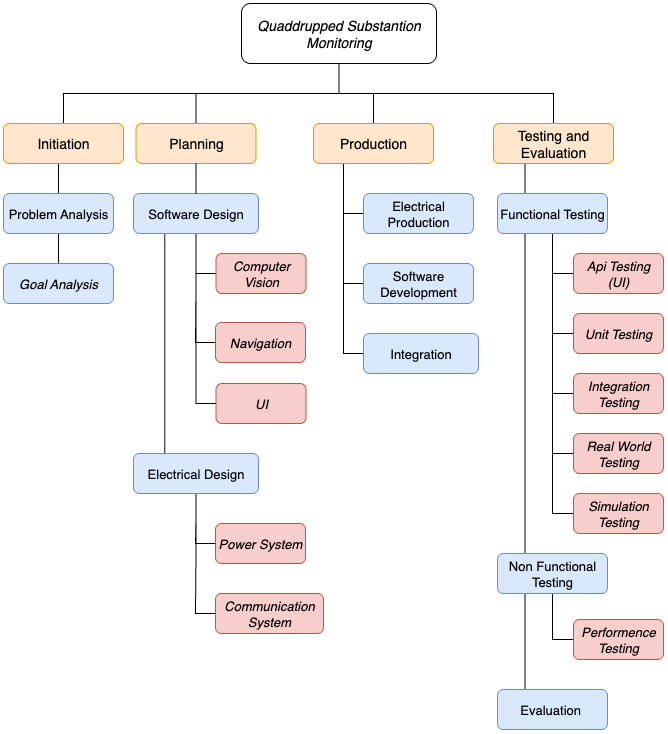
\includegraphics[width=0.85\textwidth]{gambar/bab3/wbs-ta.png}
  \caption{\emph{Work Breakdown Structure (WBS)} Penelitian}
  \label{fig:wbs}
\end{figure}

Pada gambar \ref{fig:wbs} struktur pengembangan sistem \emph{Quadruped Substation Monitoring}, yang terbagi menjadi empat tahap utama, yaitu \emph{Initiation}, \emph{Planning}, \emph{Production}, dan \emph{Testing and Evaluation}. Setiap tahap memiliki elemen-elemen yang lebih spesifik yang mendetailkan proses yang terlibat. Pada tahap \emph{Initiation}, dilakukan analisis terhadap kondisi eksisting, identifikasi masalah, dan penentuan deskripsi hasil yang diinginkan dari sistem yang akan dibangun. Proses ini merupakan fondasi awal untuk memastikan bahwa tujuan yang ingin dicapai jelas dan terukur. Selanjutnya, pada tahap \emph{Planning}, dilakukan perencanaan teknis yang mencakup desain kelistrikan dan perangkat lunak. Tahap ini melibatkan berbagai aspek, seperti pengembangan sistem komunikasi dan sistem daya, yang mendukung operasi sistem secara keseluruhan. Setelah tahap perencanaan selesai, tahap \emph{Production} dimulai, yang mencakup produksi kelistrikan dan pengembangan perangkat lunak. Proses ini juga melibatkan integrasi seluruh komponen sistem untuk memastikan semuanya berjalan sesuai rencana. Pada akhirnya, pada tahap \emph{Testing and Evaluation}, sistem diuji dengan berbagai metode, baik uji fungsional seperti \emph{API Testing} dan \emph{Unit Testing}, maupun uji non-fungsional seperti \emph{Performance Testing}. Evaluasi dilakukan untuk memastikan bahwa sistem yang dibangun memenuhi standar dan tujuan yang telah ditentukan. Diagram ini secara keseluruhan membantu menggambarkan bagaimana tahapan-tahapan dalam pengembangan sistem dibagi menjadi unit-unit yang lebih kecil untuk memastikan manajemen yang lebih baik, pemantauan yang efisien, dan pengelolaan sumber daya yang optimal dalam setiap fase pengembangan.


\section{Desain Pengembangan Sistem}
Pengembangan dalam penelitian ini bertujuan untuk melakukan otomatisasi proses pemantauan suhu komponen gardu induk yang sebelumnya dilakukan secara manual, dengan memanfaatkan robot berkaki empat \emph{(quadruped-legged)} Deep Robotics X30 Pro. Agar sistem mampu melakukan pemantauan secara otomatis, diperlukan pengembangan lebih lanjut dari kondisi robot yang ada saat ini. Pengembangan sistem ini mencakup tiga tujuan utama, yaitu: sistem deteksi suhu komponen, sistem navigasi otonom, dan sistem \emph{control station}. Melalui pengembangan ini, diharapkan robot dapat melakukan patroli secara mandiri di area gardu induk, mendeteksi komponen yang mengalami kondisi \emph{overheat}, serta menyampaikan informasi yang relevan kepada operator melalui sistem \emph{control station}. Dalam proses pengembangan ini, selain dilakukan pengembangan perangkat lunak robot, juga dilakukan integrasi perangkat keras tambahan seperti kamera termal, modul komunikasi nirkabel, dan perangkat lunak sebagai sistem \emph{control station} yang akan digunakan untuk memantau kondisi robot dan memberikan informasi terkait potensi \emph{overheat} secara \emph{real-time}. Sistem \emph{control station} ini dirancang untuk memungkinkan pengawasan yang lebih efisien dan pengambilan keputusan yang lebih cepat oleh operator, dengan menggunakan data yang diperoleh dari sensor termal robot yang dipantau terus menerus. Robot tidak hanya bertugas untuk mendeteksi suhu, tetapi juga harus memiliki kemampuan navigasi yang baik untuk bergerak secara otonom di area gardu induk yang kompleks, sehingga pengembangan sistem navigasi otonom juga menjadi bagian yang sangat penting dalam penelitian ini. 


\subsection{Desain Elektrikal}

Desain elektrikal robot mencakup perancangan sistem distribusi daya dan komunikasi yang bertujuan untuk mengintegrasikan komponen-komponen tambahan ke dalam sistem robot yang telah ada. Komponen tambahan ini dirancang untuk mendukung kapabilitas operasi otonom robot secara menyeluruh. Rancangan lengkap dari sistem dapat dilihat pada Gambar~\ref{fig:electrical}.

\begin{figure}[H]
  \centering
  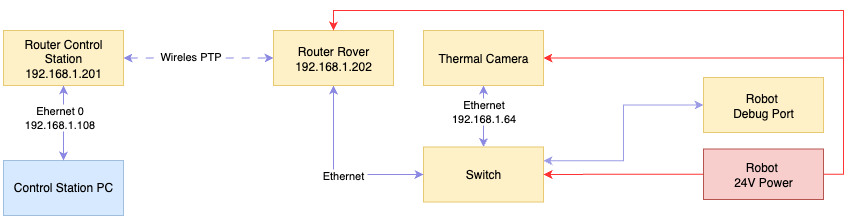
\includegraphics[width=0.85\textwidth]{gambar/bab3/electrical-design.png}
  \caption{Desain Elektrikal Robot}
  \label{fig:electrical}
\end{figure}

Pada Gambar~\ref{fig:electrical}, ditunjukkan bahwa robot dilengkapi dengan sejumlah komponen tambahan guna mendukung fungsi pemantauan suhu secara otomatis. Komponen-komponen tersebut antara lain meliputi kamera termal Hikvision HM-TD5528T-15/W, router Doublecom DB6000FR-ANS, dan perangkat \emph{switch} jaringan. Seluruh perangkat tambahan ini memerlukan catu daya sebesar 24~VDC yang disuplai langsung dari port daya pada \emph{navigation host} robot, sehingga tidak memerlukan sumber daya eksternal tambahan. Dari sisi komunikasi internal, seluruh perangkat jaringan di dalam robot terhubung melalui \emph{switch} jaringan yang kemudian diintegrasikan ke dalam sistem utama robot melalui \emph{debug port}. Konfigurasi ini membentuk suatu jaringan lokal tertutup \emph{(closed local network)}. Untuk mendukung komunikasi eksternal antara robot dan sistem \emph{control station}, digunakan skema komunikasi nirkabel \emph{Point-to-Point} (PTP) pada frekuensi 5{,}8~GHz. Dalam konfigurasi ini, perangkat pemancar yang terpasang pada \emph{control station} (Doublecom DB6000ANLT90-FR) dikonfigurasi sebagai \emph{access point} (AP), sedangkan perangkat penerima yang berada pada sisi robot berfungsi sebagai \emph{station}. Skema ini memungkinkan terjadinya pertukaran data dua arah berkecepatan tinggi dengan latensi rendah, yang sangat krusial untuk mendukung transmisi data secara \emph{real-time}, 


\subsection{Desain Sistem \emph{Computer Vision}}

Sistem \emph{computer vision} yang dikembangkan bertujuan untuk mendeteksi jenis komponen gardu induk serta menganalisis suhunya guna mengidentifikasi potensi \emph{overheat}. Proses ini dilakukan melalui dua tahap utama, yaitu deteksi objek menggunakan model \emph{YOLO} dan deteksi suhu dari komponen yang terdeteksi. Deteksi objek pada citra termal dilakukan menggunakan model \emph{YOLOv8}, model ini dipilih karena kemampuannya dalam melakukan deteksi objek secara akurat dan cepat. Hal ini penting agar suhu tinggi yang terdeteksi benar-benar berasal dari komponen gardu, dan bukan objek lain di latar. Jika terdapat objek yang dideteksi, maka dilakukan konversi citra termal ke citra skala abu-abu (\emph{grayscale}) untuk memungkinkan pemetaan suhu berdasarkan intensitas piksel. Pemetaan suhu dilakukan dengan mengubah nilai intensitas piksel citra \emph{grayscale} menjadi nilai suhu aktual berdasarkan data konfigurasi suhu minimum dan maksimum yang diperoleh melalui ISAPI. Nilai suhu aktual dari area pada \emph{bounding box} hasil deteksi objek kemudian dibandingkan dengan ambang batas suhu berdasarkan jenis komponen. Jika melebihi batas tersebut, sistem menyimpulkan adanya potensi \emph{overheat}.

\subsection{Desain Perangkat Lunak Robot}
Desain perangkat lunak pada robot dilakukan dengan mempertimbangkan arsitektur perangkat lunak yang bersifat modular dan terintegrasi. Pendekatan ini bertujuan untuk mempermudah proses pengembangan, pemeliharaan, serta pengujian sistem secara menyeluruh. Dalam penelitian ini, perangkat lunak dibagi menjadi beberapa \textit{package} ROS yang masing-masing memiliki fungsi spesifik dan saling terhubung.

Terdapat empat \textit{package} utama yang dikembangkan, yaitu \textit{IO package}, \textit{Localization and Mapping package}, \textit{Autonomy package}, dan \textit{Perception package}. Struktur umum dari arsitektur perangkat lunak ini dapat dilihat pada Gambar~\ref{fig:software-arch}.

\begin{figure}[H]
  \centering
  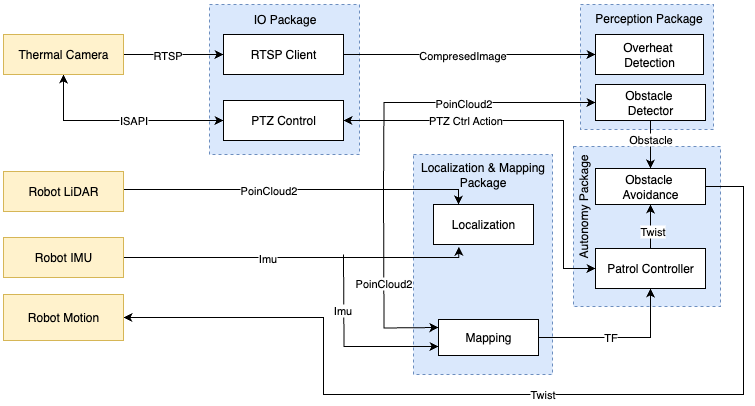
\includegraphics[width=0.8\textwidth]{gambar/bab3/sotware-arch.png}
  \caption{Arsitektur Perangkat Lunak Robot}
  \label{fig:software-arch}
\end{figure}

Pada gambar \ref{fig:software-arch} terdapat empat \emph{package} utama. \emph{IO package} mengelola komunikasi dengan perangkat keras seperti kamera thermal dan kontrol \emph{PTZ}. \emph{Localization and Mapping package} bertanggung jawab untuk pemetaan dan penentuan posisi robot menggunakan data dari sensor LiDAR dan IMU. \emph{Autonomy package} mengatur penghindaran rintangan dan kontrol patroli robot untuk navigasi otonom. \emph{Perception package} mendeteksi suhu \emph{overheat} menggunakan kamera thermal dan membantu robot dalam mengidentifikasi hambatan Setiap \textit{package} menjalankan fungsi tertentu dan saling berkomunikasi melalui mekanisme \textit{topic}, \textit{service}, atau \textit{action} sesuai dengan kebutuhan sistem.

\subsubsection{3.2.3.1 \emph{IO Package}}
\textit{IO package} bertanggung jawab untuk mengelola seluruh input dan output dari perangkat keras robot, yang dalam hal ini adalah kamera thermal. \textit{IO package} terdiri dari dua program utama, yaitu \textit{RTSP client} dan \textit{PTZ controller}.  \textit{RTSP client} berfungsi untuk menghubungkan kamera thermal dengan sistem robot dan mengubah aliran data menjadi \textit{rostopic} berupa \textit{compressed image}. Sementara itu, \textit{PTZ controller} digunakan untuk mengatur pergerakan \textit{pan-tilt-zoom (PTZ)} serta menerima status posisi \emph{PTZ} saat ini menggunakan protokol \emph{ISAPI}. Informasi ini kemudian digunakan untuk mengontrol pergerakan \emph{PTZ} secara dinamis, yang dipadukan dengan \textit{PID controller} untuk memperoleh kecepatan rotasi dan sudut target yang akurat.

\subsubsection{3.2.3.2 \emph{Localization and Mapping Package}}
\emph{Localization and Mapping Package} bertanggung jawab untuk melakukan estimasi posisi robot secara \emph{real-time} di dalam lingkungan serta memperbarui peta berdasarkan data sensor yang diterima. Dalam penelitian ini, sistem memanfaatkan empat buah sensor LiDAR Livox Mid-360 dan satu unit Yesense-IMU sebagai sumber data utama. Sistem ini mengimplementasikan berbagai metode \emph{localization} yang mencakup pendekatan berbasis \emph{odometry-only} maupun pendekatan berbasis \emph{Simultaneous Localization and Mapping} (SLAM). Dua metode pertama merupakan metode berbasis \emph{odometry-only}, yaitu \emph{FastLIO2} dan \emph{DLIO} (\emph{Direct LiDAR-Inertial Odometry}), yang melakukan estimasi posisi robot secara langsung berdasarkan integrasi data LiDAR dan IMU tanpa melakukan pemetaan lingkungan. Karena tidak membentuk peta, metode ini memiliki keterbatasan dalam hal inisialisasi di mana proses \emph{localization} harus selalu dimulai dari posisi awal yang sama setiap kali sistem dijalankan, sehingga tidak adaptif terhadap perubahan posisi awal robot. 

Metode ketiga dan keempat menggunakan konsep pemisahan antara proses \emph{mapping} dan \emph{localization} yang tetap terintegrasi sesuai prinsip \emph{frontend-backend} dalam sistem SLAM modern. Pada metode ketiga proses pemetaan dilakukan menggunakan \emph{FastLIO2} untuk menghasilkan representasi peta dua dimensi dalam bentuk \emph{grid-map}, yang kemudian dimanfaatkan oleh \emph{HDL Localization} untuk melakukan proses pelokalan. Pendekatan keempat menggunakan metode \emph{Fast-LIO-SAM} yang menggabungkan estimasi \emph{LiDAR-Inertial Odometry} (LIO) pada \emph{frontend} dengan proses optimisasi graf berbasis \emph{Smoothing and Mapping} (SAM) pada \emph{backend}, menghasilkan peta lingkungan tiga dimensi dalam format file \texttt{.bag} yang kemudian digunakan oleh \emph{Fast-LIO Localization QN} untuk proses \emph{localization}. Pada metode ketiga dan keempat, proses \emph{mapping} dan \emph{localization} tidak berjalan secara bersamaan sehingga memerlukan peta hasil pemetaan yang telah tersedia sebelum proses \emph{localization} dijalankan. Koordinat posisi robot yang dihasilkan dipublikasikan ke dalam sistem ROS melalui transformasi koordinat menggunakan modul \emph{tf broadcaster}.

\subsubsection{3.2.3.1 \emph{Perception Package}}
\emph{Perception package} bertanggung jawab untuk melakukan estimasi posisi komponen yang mengalami panas berlebih (\emph{overheat}) pada gardu induk. Proses ini dilakukan dengan meimplementasikan sistem \emph{computer vision} yang telah dijelaskan pada subbab 3.2.1.  Selain itu \emph{Perception package} juga mengelola deteksi rintangan yang dilakukan oleh robot. Sistem ini menggunakan algoritma \emph{Braitenberg} untuk mendeteksi dan menghindari rintangan di sekitar robot. Deteksi rintangan dilakukan dengan memanfaatkan sensor LiDAR yang terpasang pada robot, yang menghasilkan garis deteksi rintangan dalam sudut 180 derajat dari sisi kiri ke arah depan robot. Setiap garis deteksi memiliki bobot atau nilai \emph{multiplier} yang berbeda, yang digunakan untuk menilai tingkat risiko dan menentukan keputusan gerakan robot. Hasil  deteksi rintangan, akan diteruskan ke \emph{autonomy package} sebagai masukan untuk pengambilan keputusan navigasi secara otonom. Dengan pendekatan ini, sistem mampu melakukan deteksi serta identifikasi objek secara efisien, dan memberikan kontribusi penting dalam memastikan keselamatan serta efektivitas pergerakan robot di lingkungan nyata.

\subsubsection{3.2.3.2 \emph{Autonomy Package}}
Dalam sistem \emph{autonomy}, yang pada dasarnya merupakan proses navigasi jalur, lintasan robot diperoleh dari hasil perekaman \emph{path} yang dilakukan secara manual. Jalur ini kemudian disimpan dalam format \texttt{.json}. pada database \emph{control station}. Integrasi antara pengendalian lintasan dan penghindaran rintangan menjadi aspek yang krusial dalam sistem ini. Salah satu strategi yang umum digunakan adalah mengimplementasikan algoritma \emph{PID Pure Pursuit} sebagai pengendali utama lintasan, sementara modul penghindaran rintangan berbasis \emph{Braitenberg} diaktifkan secara kondisional ketika objek terdeteksi dalam jarak tertentu. Pendekatan ini memungkinkan robot untuk tetap mengikuti jalur yang telah direkam, namun tetap mampu bereaksi secara dinamis terhadap rintangan tanpa harus melakukan perencanaan ulang lintasan secara menyeluruh. Integrasi semacam ini dapat direalisasikan melalui skema \emph{behavior-based arbitration} atau \emph{subsumption architecture}, di mana modul penghindaran rintangan memiliki prioritas lebih tinggi ketika kondisi kritis terdeteksi. Setelah lingkungan kembali aman, kontrol akan dialihkan kembali ke pengendali lintasan utama. Selain navigasi jalur \emph{autonomy package} juga mengelola proses pengambilan gambar dari kamera termal yang terpasang pada robot. Proses ini dilakukan jika robot telah sampai pada titik koordinat tertentu yang telah ditentukan sebelumnya sistem akan mengirim perintah ke \emph{IO package} untuk mengerakan kamera termal ke posisi yang telah ditentukan. Setelah kamera berada pada posisi yang tepat, \emph{IO package} akan mengirim perintah ke \emph{RTSP client} untuk mengambil gambar dimana gambar yang diambil akan dikirim ke \emph{perception package} untuk dilakukan deteksi objek dan analisis suhu. 

\subsection{Desain \textit{Control Station}}

Sistem ini dirancang layaknya sebuah \emph{fleet management system} yang bertugas untuk memantau dan mengatur seluruh aktivitas operasional robot di lapangan secara \emph{real-time}. Fungsi utama dari sistem ini mencakup pemantauan posisi robot secara langsung pada peta, penyajian hasil deteksi suhu komponen serta visualisasi potensi \emph{overheat} pada komponen gardu, akses terhadap tampilan kamera langsung (\emph{live camera}), serta pengaturan dan penjadwalan jalur patroli. Perancangan \emph{control station} ini mengadopsi pendekatan berbasis web, sehingga dapat diakses dari berbagai perangkat secara fleksibel tanpa memerlukan instalasi tambahan. Hal ini penting untuk mendukung kebutuhan mobilitas operator di lapangan. 

\subsubsection{3.2.4.1 Perancangan \emph{User Interface}}

Tahap ini mencakup desain visual antarmuka, termasuk tata letak, elemen grafis, serta skema warna yang digunakan dalam sistem. Desain UI harus mempertimbangkan prinsip \emph{usability} dan \emph{user experience}, seperti konsistensi, umpan balik sistem, dan efisiensi interaksi. Selain itu, aspek estetika juga diperhatikan untuk mendukung kenyamanan visual dalam penggunaan jangka panjang. Penempatan elemen dirancang agar informasi kritis, seperti posisi robot, suhu komponen, dan status kamera, dapat diakses dengan cepat.Antarmuka juga dirancang agar mendukung tampilan multi-robot, memungkinkan operator memantau beberapa unit secara bersamaan. Navigasi antarmuka menggunakan pendekatan berbasis tab untuk menjaga keteraturan informasi. Berikut adalah desain antarmuka \emph{control station} yang telah dirancang:

\begin{figure}[H]
  \centering
  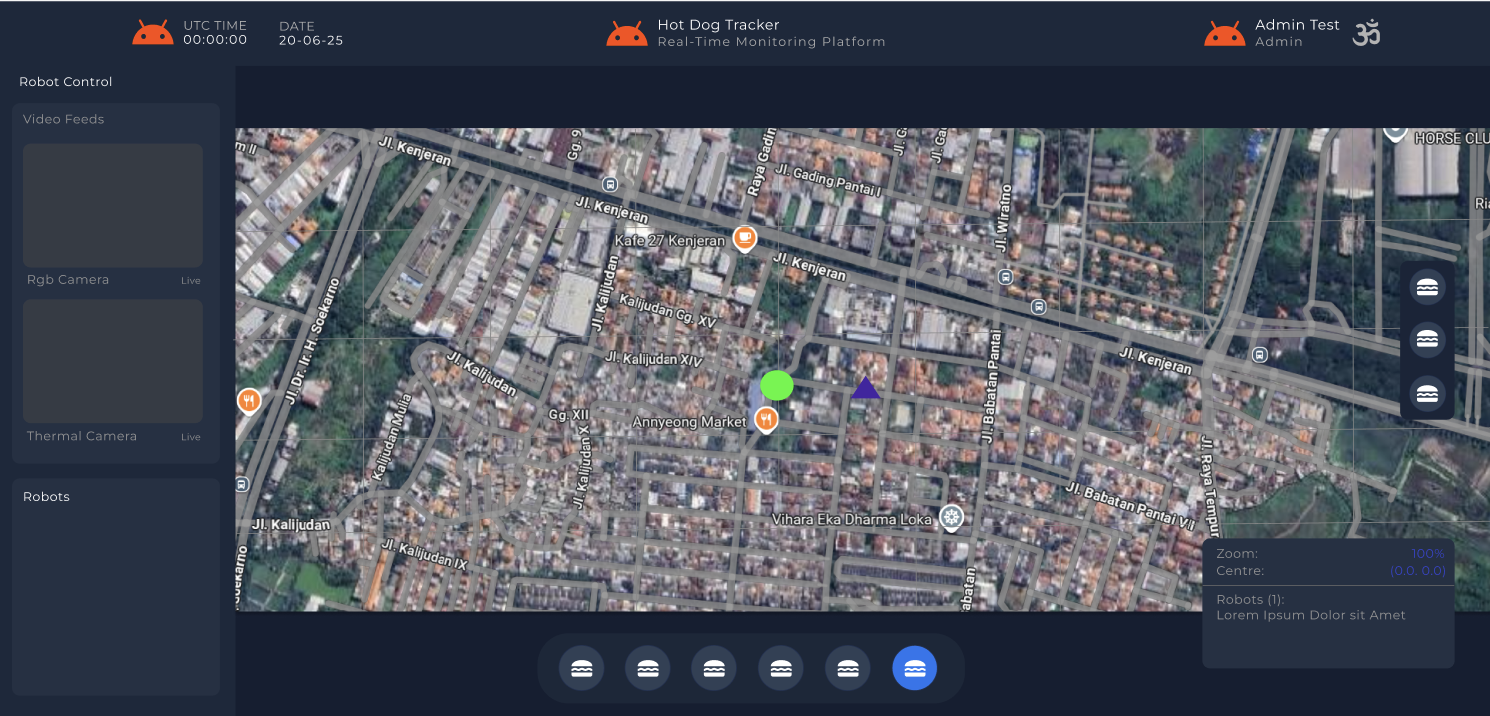
\includegraphics[width=0.84\textwidth]{gambar/bab3/home-fix.png}
  \caption{Desain halaman utama pada \emph{control station}}
  \label{fig:control-station-robot-main}
\end{figure}


Pada Gambar~\ref{fig:control-station-robot-main}, terlihat bahwa halaman utama \emph{control station} menampilkan peta yang menunjukkan posisi robot secara \emph{real-time}. Peta ini dilengkapi dengan informasi terkait suhu komponen yang terdeteksi, serta status kamera termal. Selain itu, terdapat juga fitur untuk mengakses tampilan kamera langsung (\emph{live camera}) dan pengaturan jalur patroli. Antarmuka dirancang agar mudah dinavigasi, dengan elemen-elemen yang jelas dan responsif terhadap interaksi pengguna. Hal ini bertujuan untuk memastikan operator dapat dengan cepat memahami kondisi lapangan dan mengambil tindakan yang diperlukan. Selain halaman utama, dalam \emph{control station} juga terdapat beberapa halaman lain seperti halaman \emph{overheat component}


\begin{figure}[H]
  \centering
  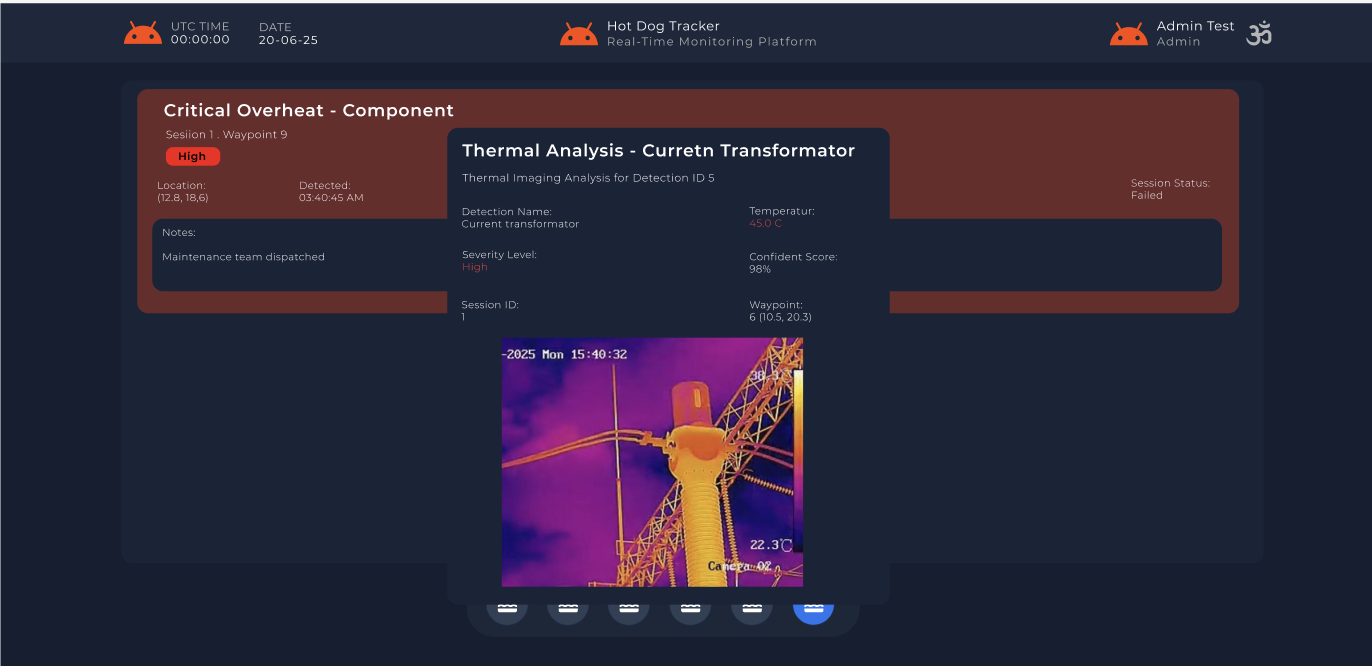
\includegraphics[width=0.84\textwidth]{gambar/bab3/overheat.png}
  \caption{Desain halaman \emph{overheat component} pada \emph{control station}}
  \label{fig:control-station-overheat}
\end{figure}


Pada Gambar~\ref{fig:control-station-overheat}, ditampilkan antarmuka halaman \emph{Overheat Component} yang berfungsi untuk menampilkan daftar komponen gardu induk yang terdeteksi mengalami suhu berlebih. Setiap entri pada daftar ini mencakup informasi penting seperti jenis komponen, lokasi keberadaan komponen, serta nilai suhu yang terdeteksi secara real-time oleh kamera termal. Halaman ini dirancang untuk menyajikan informasi secara jelas, ringkas, dan mudah dipahami oleh operator, sehingga memungkinkan pengambilan keputusan secara cepat untuk mencegah potensi kerusakan lebih lanjut pada komponen penting sistem kelistrikan. 
Sistem \emph{Control Station} juga menyediakan sejumlah halaman pendukung lainnya yang bertujuan untuk mempermudah proses manajemen data dan pengoperasian sistem secara keseluruhan. Halaman \emph{Robot Management} digunakan untuk mengelola data robot, termasuk identitas, status operasional, serta konfigurasi parameter. Halaman \emph{Component Management} digunakan untuk mencatat dan memperbarui informasi mengenai komponen-komponen gardu induk yang dimonitor. Sementara itu, halaman \emph{Patrol Management} berfungsi untuk menyusun, menjadwalkan, dan memantau pelaksanaan rute patroli robot secara otomatis. Selanjutnya, tersedia pula halaman \emph{User Management} yang digunakan untuk mengelola data pengguna, hak akses, serta otentikasi sistem, dan halaman \emph{System Configuration} yang berfungsi untuk mengatur berbagai parameter sistem seperti koneksi jaringan, waktu sistem, dan pengaturan integrasi perangkat. Seluruh halaman ini dirancang dengan prinsip kemudahan penggunaan (\emph{user-friendly}) dan konsistensi antarmuka, guna memastikan operator dapat mengakses dan mengelola data secara efisien. Tampilan rancangan antarmuka pengguna secara lebih rinci dapat dilihat pada Lampiran~1 berjudul \emph{Design UI/UX Control Station}.



\subsubsection{3.2.4.2 \emph{Physical data model design}}
\emph{Physical data model design} berfokus pada strukturisasi dan organisasi data yang akan dikelola oleh sistem. Ini meliputi definisi entitas data seperti data robot, komponen gardu, route, riwayat patroli, user, dan informasi konfigurasi sistem. Perancangan ini juga mencakup penetapan relasi antar entitas dan tipe data untuk memastikan integritas dan efisiensi penyimpanan serta pengambilan data. Adapun \emph{physical data model} yang digunakan dalam sistem ini dapat dilihat pada Gambar~\ref{fig:physical-data-model}.

\begin{figure}[H]
  \centering
  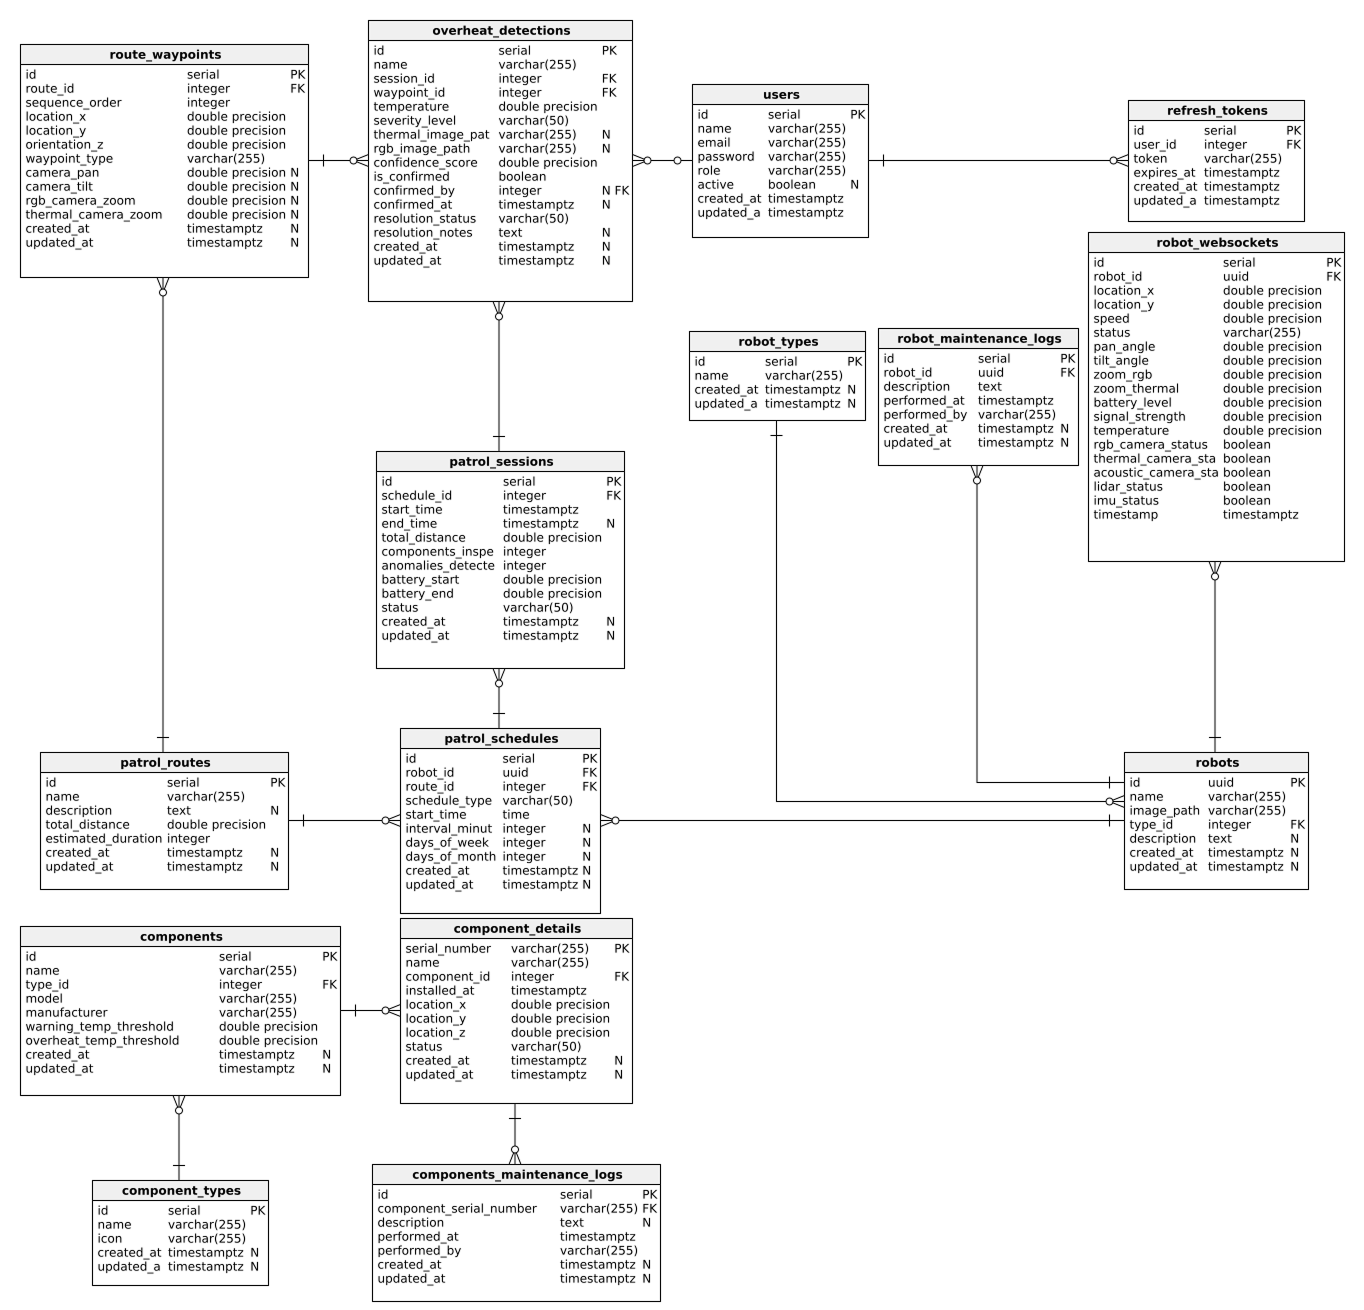
\includegraphics[width=0.87\textwidth]{gambar/bab3/pdm.png}
  \caption{\emph{Physical Data Model} \emph{Control Station}}
  \label{fig:physical-data-model}
\end{figure}

Dari \emph{physical data model} yang ditunjukkan pada Gambar~\ref{fig:physical-data-model}, terlihat adanya sejumlah entitas utama seperti \emph{robots}, \emph{patrol\_routes}, \emph{patrol\_schedules}, dan \emph{patrol\_sessions} yang merepresentasikan proses penjadwalan serta pelaksanaan patroli robot secara sistematis.  Entitas \emph{components} dan \emph{component\_details} digunakan untuk menyimpan data komponen gardu induk yang dimonitor, termasuk informasi jenis komponen, lokasi pemasangan, serta parameter ambang batas suhu abnormal yang menjadi indikator potensi gangguan. Informasi mengenai jenis komponen tersebut direferensikan melalui entitas \emph{component\_types}. Proses deteksi suhu berlebih atau potensi kondisi \emph{overheat} dicatat dalam entitas \emph{overheat\_detections}, yang memiliki relasi dengan sesi patroli pada entitas \emph{patrol\_sessions} dan data komponen terkait pada entitas \emph{components}. Dengan demikian, setiap deteksi dapat ditelusuri berdasarkan sesi inspeksi dan lokasi komponen secara historis. Posisi dan status robot secara waktu nyata dikelola melalui entitas \emph{robot\_websockets}, yang mencatat data seperti koordinat posisi, arah hadap, status sensor, serta kekuatan sinyal komunikasi nirkabel. Informasi jenis robot tersimpan dalam entitas \emph{robot\_types}, yang merepresentasikan klasifikasi atau spesifikasi teknis masing-masing unit robot. Sistem ini juga mendukung pengelolaan pengguna melalui entitas \emph{users} dan \emph{refresh\_tokens} yang digunakan dalam mekanisme autentikasi dan otorisasi akses sistem. Dengan penerapan manajemen token, keamanan dan validitas sesi pengguna dapat dikontrol secara efektif. Relasi antar entitas pada \emph{physical data model} ini dirancang untuk mendukung integritas data, konsistensi referensial, serta efisiensi dalam operasional sistem pemantauan dan pengendalian robot. Detail struktur tabel beserta relasi antar entitas dapat dilihat pada Lampiran~2 \emph{Database Model Documentation}.

\subsubsection{3.2.4.3 \emph{Use case diagram}}
\emph{Use case diagram} digunakan untuk menggambarkan interaksi antara pengguna (aktor) dengan sistem. Diagram ini membantu dalam memahami kebutuhan fungsional sistem dan bagaimana pengguna akan berinteraksi dengan berbagai fitur yang disediakan. Berikut adalah \emph{use case diagram} yang menggambarkan interaksi antara pengguna dengan sistem \emph{control station}:

\begin{figure}[H]
  \centering
  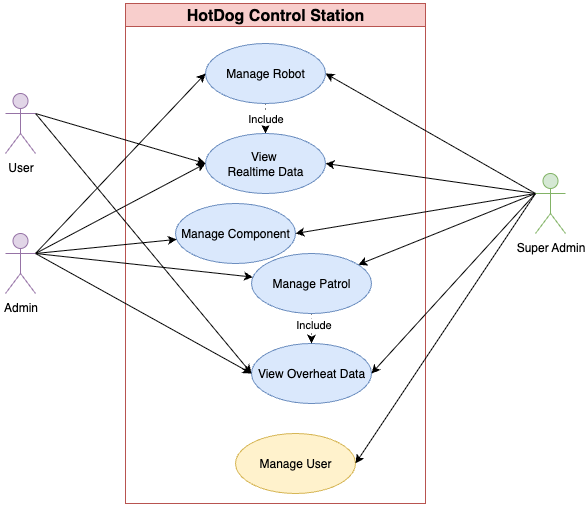
\includegraphics[width=0.85\textwidth]{gambar/bab3/usecase.png}
  \caption{\emph{Use Case Diagram} \emph{Control Station}}
  \label{fig:use-case-diagram}
\end{figure}

Pada Diagram~\ref{fig:use-case-diagram}, terdapat tiga aktor utama, yaitu \emph{User}, \emph{Admin}, dan \emph{Super Admin}, yang masing-masing memiliki tingkat akses yang berbeda terhadap sistem. Aktor \emph{User} hanya memiliki akses terbatas, yaitu untuk melihat data posisi dan data robot secara waktu nyata melalui fitur \emph{View Realtime Data}, serta mengakses informasi suhu berlebih melalui fitur \emph{View Overheat Data}. Sementara itu, aktor \emph{Admin} memiliki cakupan akses yang lebih luas, mencakup pengelolaan data robot, data komponen gardu, serta penjadwalan patroli robot. Selain itu, \emph{Admin} juga memiliki hak untuk melihat data anomali suhu, namun tidak diberi wewenang untuk melakukan pengelolaan pengguna dalam sistem. Akses penuh terhadap seluruh fitur sistem, termasuk kemampuan untuk mengelola pengguna melalui fitur \emph{Manage User}, hanya dimiliki oleh aktor \emph{Super Admin}. Dalam struktur hierarki ini, fitur \emph{View Realtime Data} merupakan bagian dari proses \emph{Manage Robot}, sedangkan fitur \emph{View Overheat Data} termasuk dalam cakupan \emph{Manage Patrol}.Dengan pembagian peran dan hak akses yang jelas ini, sistem dirancang untuk memastikan kontrol yang terstruktur dan keamanan data operasional yang optimal.


\section{Implementasi Sistem}
\sloppy
Implementasi sistem dilakukan dengan meimplementasikan rancangan yang telah dibuat pada tahap sebelumnya. Proses implementasi ini mencakup pengembangan perangkat lunak robot, integrasi perangkat keras, serta pengembagan sistem \emph{control station}.

\subsection{Implementasi Sistem \emph{Electrical}}
Implementasi sistem elektrikal dilakukan dengan mengintegrasikan komponen-komponen tambahan ke dalam robot yang telah ada. Proses ini meliputi pemasangan kamera termal, router nirkabel, dan perangkat \emph{switch} jaringan. Pemasangan dilakukan dengan memperhatikan skema distribusi daya yang telah dirancang sebelumnya, sehingga seluruh komponen dapat beroperasi dengan baik tanpa memerlukan sumber daya eksternal tambahan. Catu daya 24~VDC disuplai langsung dari port daya pada \emph{navigation host} robot seperti pada Gambar~\ref{fig:int-control-port}. 

\begin{figure}[H]
  \centering
  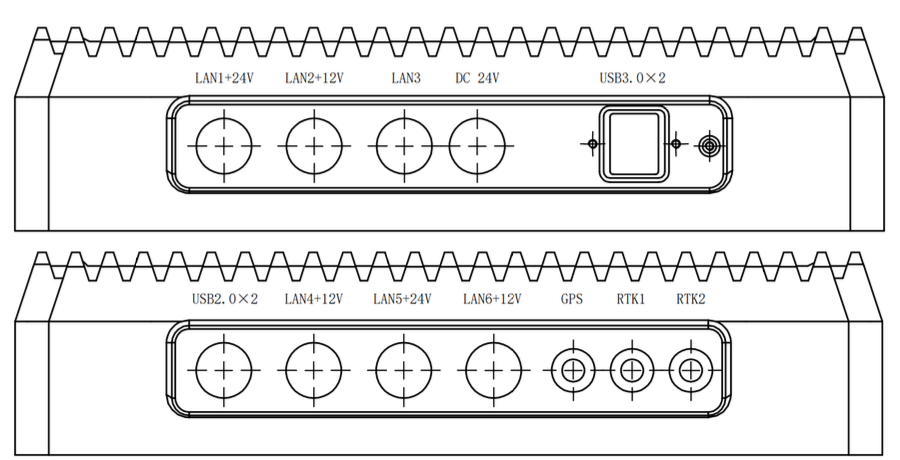
\includegraphics[width=0.8\textwidth]{gambar/bab3/int-control-port.png}
  \caption{Port pada \emph{Navigation Host} Robot  Tampak depan (A) dan belakang (B) \cite{deeprobotics_jueyingx30}}
  \label{fig:int-control-port}
\end{figure}

Berdasarkan gambar \ref{fig:int-control-port} dapat diketahui bahwa robot memiliki catu daya sebesar 24~VDC yang dapat digunakan untuk menyuplai perangkat tambahan. Berdasarkan data spesifikasi dari Deep Robotics X30 Pro, daya maksimum yang dapat disuplai oleh satu port 24~V adalah 240~W, dengan arus maksimum sebesar 10~A. Perangkat tambahan yang digunakan terdiri dari: (1) kamera termal Hikvision HM-TD5528T-15/W dengan konsumsi daya sebesar 20~W, (2) router nirkabel Doublecom DB6000FR-ANS dengan konsumsi daya maksimum kurang dari 9~W, dan (3) \emph{switch} Moxa EDS-205 dengan arus input sebesar 0{,}12~A pada tegangan 24~VDC, sehingga daya yang dibutuhkan adalah sebesar 2{,}88~W. Dengan demikian, total konsumsi daya dari seluruh perangkat tambahan adalah sekitar 31{,}88~W, yang masih berada dalam batas kemampuan suplai daya robot. Beradaskan data tersebut total daya yang dibutuhkan oleh perangkat tambahan adalah:
\[
P_{\text{total}} = 20~W + 9~W + 2{,}88~W = 31{,}88~W
\]

Jika tegangan yang digunakan konstan 24~V, maka arus yang digunakan oleh perangkat tambahan adalah:
\[
I = \frac{P_{\text{total}}}{V} = \frac{31{,}88~W}{24~V} \approx 1{,}33~A
\]

Persentase penggunaan terhadap kapasitas maksimum port adalah:
\[
\text{Daya (\%P):} \quad \frac{31{,}88}{240} \times 100\% \approx 13{,}283333333\%
\]

Dengan demikian, total konsumsi daya dan arus perangkat tambahan hanya sekitar 13{,}3\% dari kapasitas maksimum port 24~V, sehingga masih berada dalam batas aman dan tidak membebani sistem catu daya robot. Selain sistem catu daya, implementasi ini juga mencakup konfigurasi komunikasi perangkat tambahan agar dapat diakses oleh robot.  
\begin{figure}[H]
  \centering
  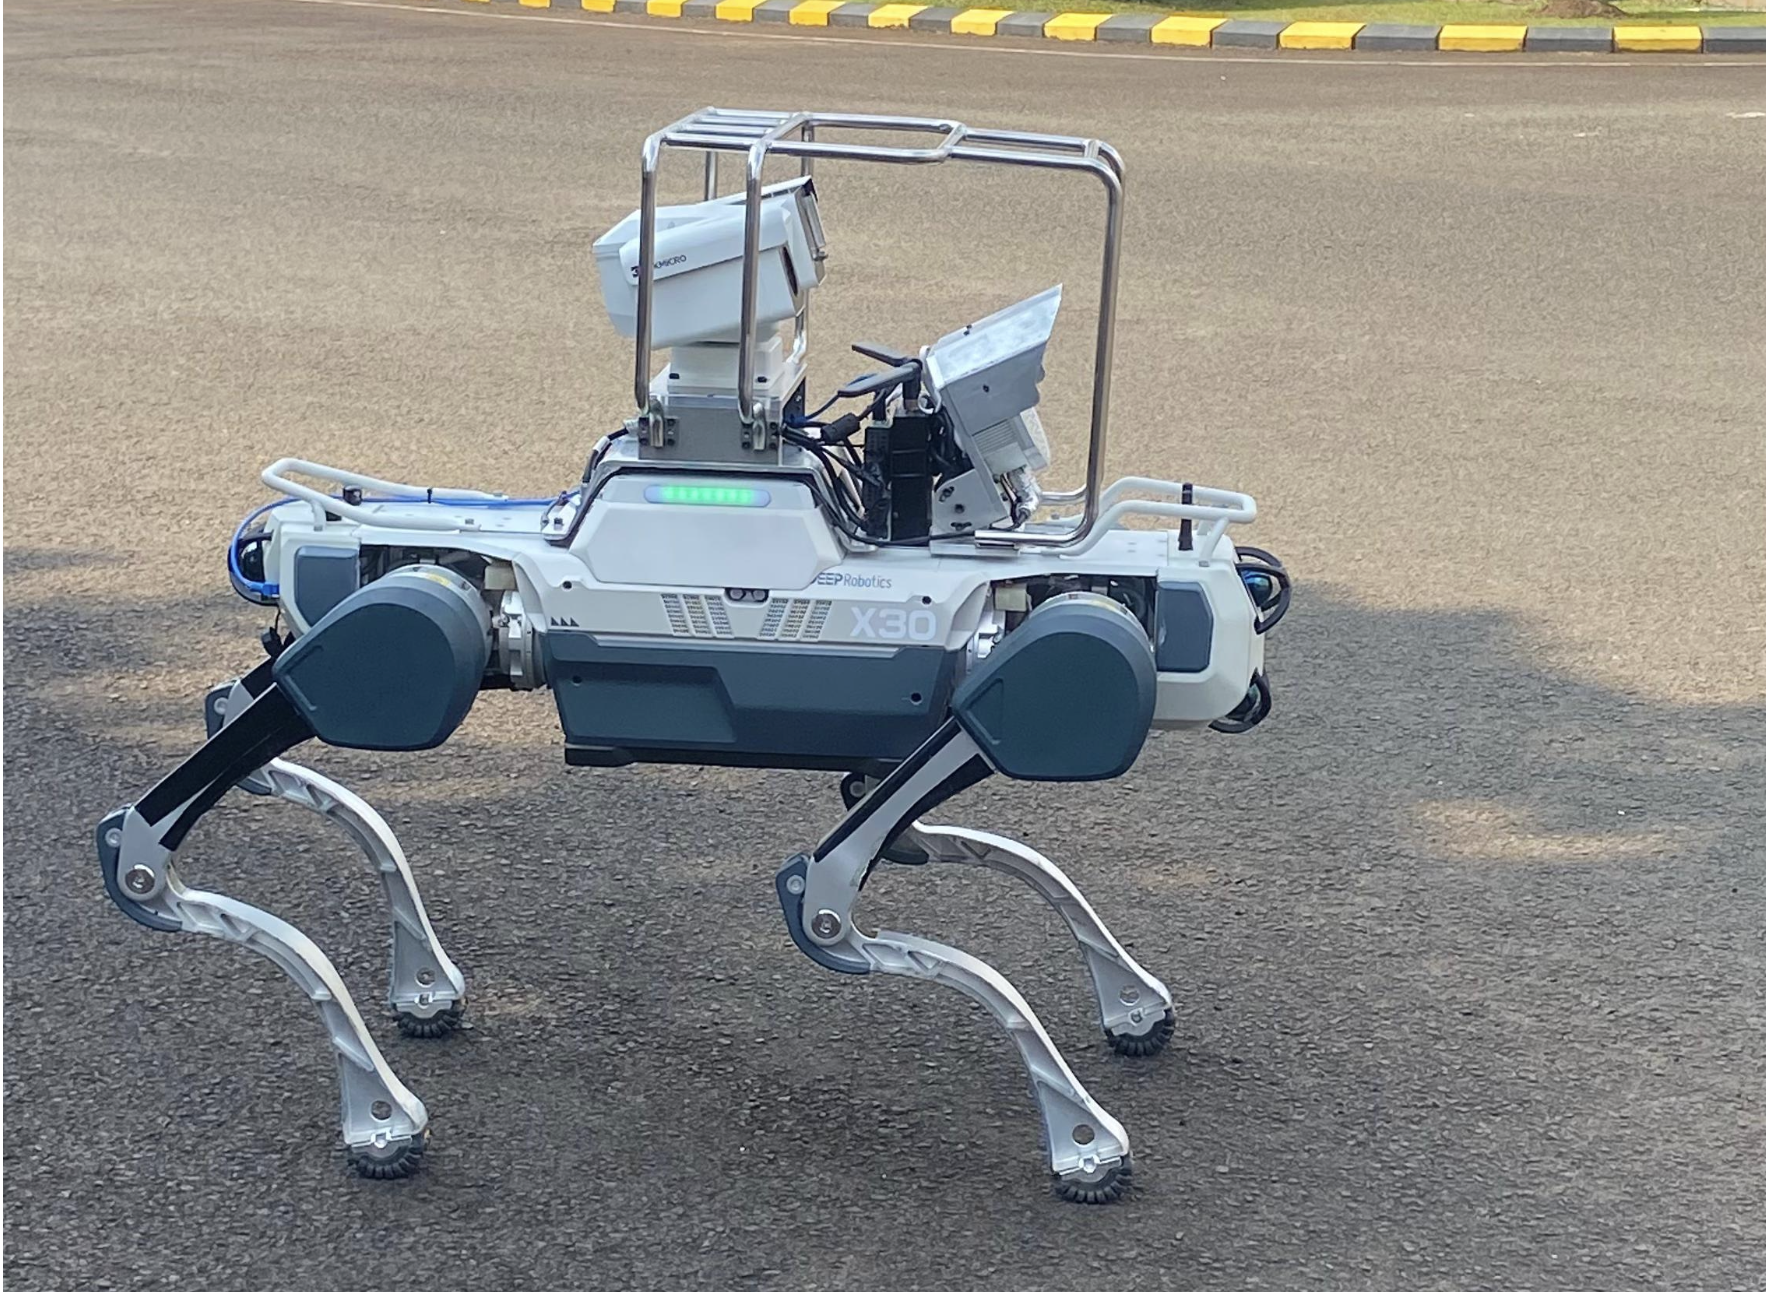
\includegraphics[width=0.8\textwidth]{gambar/bab3/impl-elec2.png}
  \caption{Integrasi robot dengan hardware external yang diperlukan}
  \label{fig:sistem-elec-robot}
\end{figure}

Dalam implementasinya, perangkat \emph{switch} Moxa yang terpasang pada robot akan dihubungkan dengan sebuah \emph{switch} eksternal yang juga terkoneksi dengan kamera termal. Semua komponen diletakan di bagian atar robot pada \emph{mounting} yang telah disediakan sebagaimana ditunjukkan pada Gambar~\ref{fig:sistem-elec-robot}. \emph{Switch} eksternal ini berfungsi sebagai penghubung antara kamera termal dengan router nirkabel yang juga dipasang pada robot. Router nirkabel tersebut menyediakan koneksi internet yang diperlukan untuk mengakses data dari kamera termal secara langsung, sekaligus menyediakan koneksi nirkabel ke \emph{control station} yang berada di luar robot. Dengan demikian, komunikasi antara robot dan sistem pengendali jarak jauh dapat dilakukan secara nirkabel. Kedua \emph{switch} tersebut kemudian dihubungkan ke port jaringan yang tersedia pada robot. Seluruh perangkat dikonfigurasi dalam satu jaringan lokal dengan skema alamat IP yang seragam, yaitu 192.168.1.\texttt{x}, sehingga memungkinkan komunikasi langsung antarperangkat tanpa melalui jaringan publik. Kamera termal diatur menggunakan alamat IP statis 192.168.1.64, dan berada dalam satu segmen jaringan yang sama dengan router dan robot. Hal ini memungkinkan pengambilan data secara langsung melalui koneksi Ethernet. 



\subsection{Implementasi sistem \emph{computer vision}}
Pada tahap implementasi sistem \emph{computer vision}, dilakukan beberapa langkah utama yang mencakup pembuatan dataset, pelatihan model deteksi objek, konversi model ke format \emph{OpenVINO}, dan inferensi model untuk mendeteksi objek serta menganalisis suhu komponen gardu induk. Proses ini bertujuan untuk mengidentifikasi komponen gardu induk yang mengalami kondisi \emph{overheat} berdasarkan citra termal yang diambil oleh kamera termal yang terpasang pada robot.


\subsubsection{3.3.2.1 Pembuatan Dataset}
Dataset citra termal yang digunakan dalam penelitian ini berasal dari dua sumber utama. Dataset pertama diperoleh dari repositori publik \emph{Roboflow Universe}, yang menyediakan citra termal berbagai komponen gardu induk, seperti \emph{arrester}, \emph{breaker}, \emph{bushing}, \emph{clamp}, \emph{conservator}, \emph{current transformer}, \emph{disconnector}, \emph{heat sink}, \emph{insulator}, dan \emph{transformer}. Dataset kedua dikumpulkan secara langsung dari GITET (Gardu Induk Tegangan Ekstra Tinggi) PLN Gandul melalui proses perekaman video menggunakan kamera termal robot. Video hasil perekaman tersebut kemudian diunggah ke platform \emph{Roboflow}, yang secara otomatis mengkonversi video menjadi kumpulan citra (frame) individual. Citra-citra inilah yang selanjutnya digunakan sebagai dasar proses anotasi. Setiap komponen pada citra termal diberi label sesuai kelasnya, seperti \emph{current transformer}, \emph{circuit breaker}, maupun PMT (Pemutus tegangan gardu) seperti ditunjukkan pada Gambar~\ref{fig:dataset-annotated}. 
\begin{figure}[H]
  \centering
  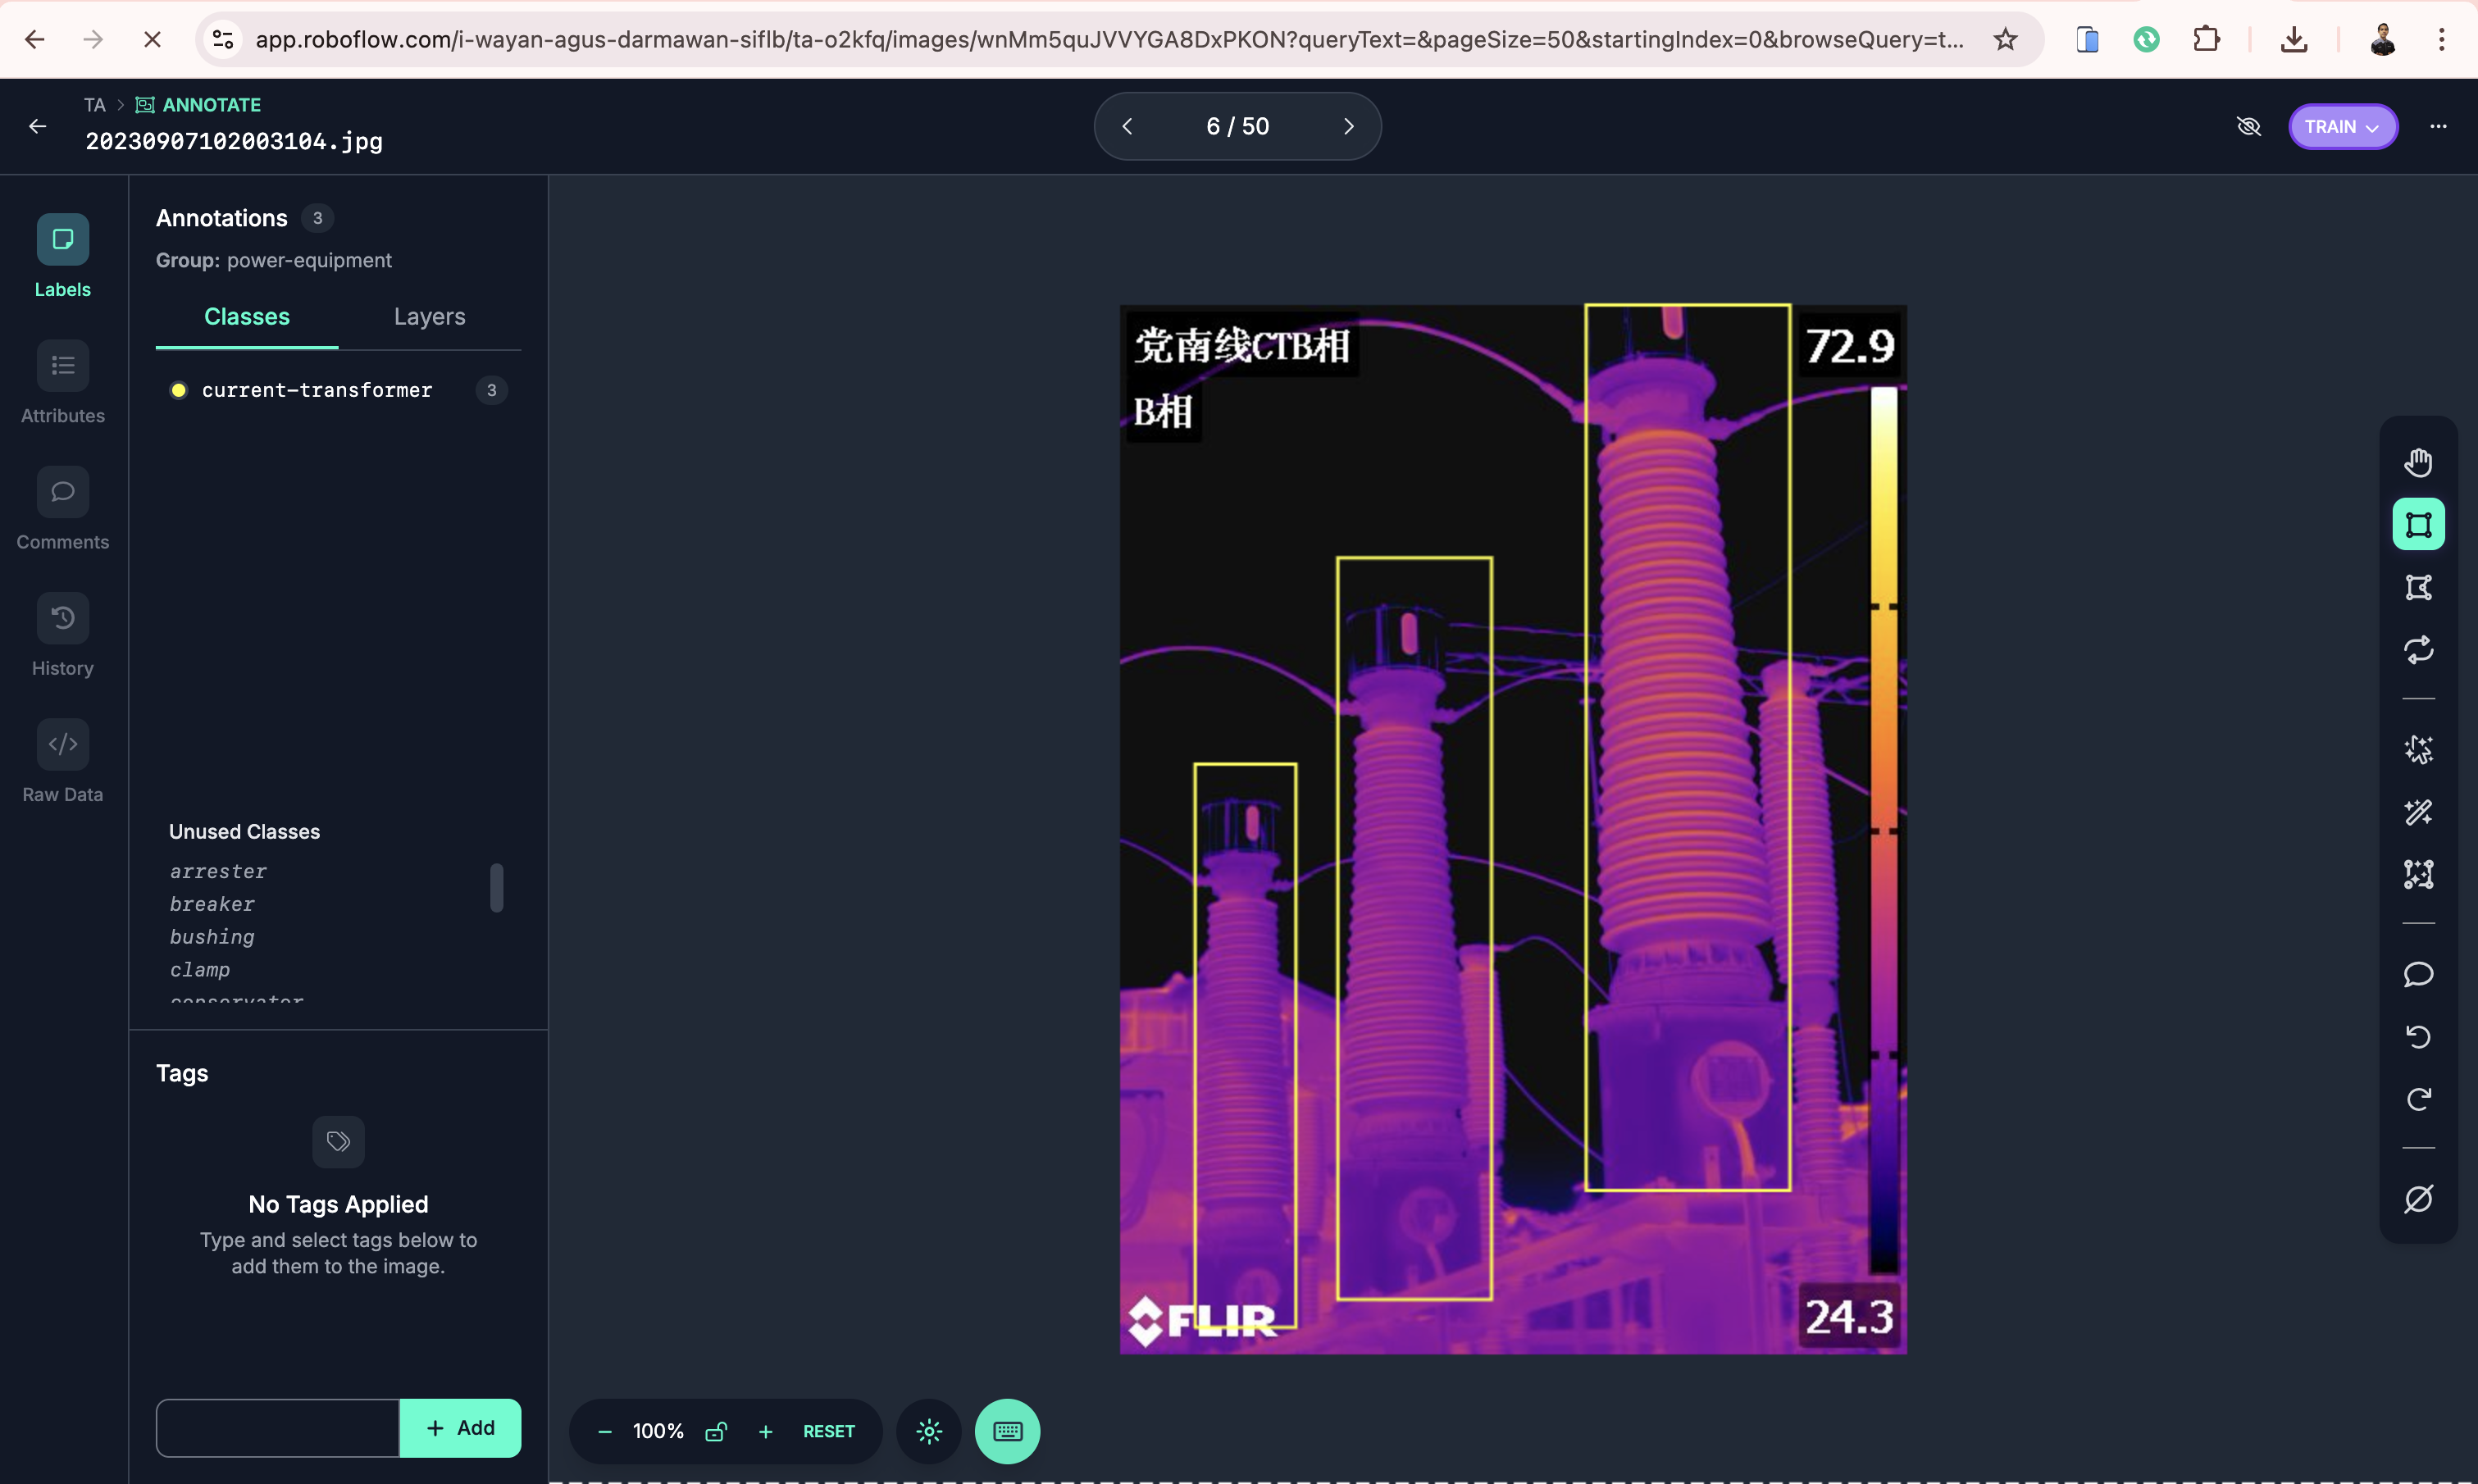
\includegraphics[width=0.7\textwidth]{gambar/bab3/dataset-anotated.png}
  \caption{Labeling dataset citra termal pada \emph{Roboflow}}
  \label{fig:dataset-annotated}
  \end{figure}

Pada Gambar~\ref{fig:dataset-annotated} terlihat contoh citra termal yang telah dianotasi dengan label yang sesuai. Proses anotasi ini dilakukan secara manual oleh peneliti dengan bantuan alat anotasi yang disediakan oleh platform \emph{Roboflow}. Proses anotasi ini krusial untuk memastikan model mampu mengenali dan mengklasifikasikan berbagai komponen gardu induk dengan akurat berdasarkan karakteristik citra termal. Dataset kemudian di bagi menjadi tiga bagian: data pelatihan, data validasi, dan data uji. Proporsi pembagian dataset adalah 70\% untuk pelatihan, 20\% untuk validasi, dan 10\% untuk pengujian. Pembagian ini bertujuan untuk memastikan model dapat belajar dengan baik dari data yang tersedia, serta menghindari overfitting pada saat pelatihan.

\subsubsection{3.3.2.2 \emph{Preprocessing} Dataset}
Dataset citra termal dikumpulkan dan dianotasi, langkah selanjutnya adalah melakukan proses \emph{preprocessing} terhadap data tersebut. Pada penelitian ini, \emph{preprocessing} dilakukan dengan mengubah ukuran citra agar sesuai dengan format input yang dibutuhkan oleh model deteksi objek. Ukuran citra yang digunakan adalah 640$\times$640 piksel, yang merupakan standar umum untuk banyak arsitektur model deteksi seperti YOLO. Dalam \emph{preprocessing} ini digunakan \emph{resize} citra dengan menggunakan \emph{Roboflow} seperti ditunjukkan pada 
Gambar~\ref{fig:dataset-resize}.

\begin{figure}[H]
  \centering
  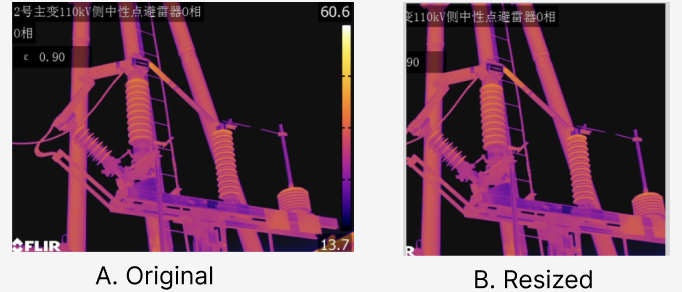
\includegraphics[width=0.7\textwidth]{gambar/bab3/prep-resize.png}
  \caption{Proses \emph{resize} dataset citra termal pada \emph{Roboflow}}
  \label{fig:dataset-resize}
\end{figure}

Gambar~\ref{fig:dataset-resize} terlihat bahwa citra awal diubah menjadi ukuran 640$\times$640 piksel dengan metode \emph{center crop}. Metode ini memastikan bahwa citra tetap mempertahankan proporsi aslinya dengan memotong bagian yang tidak diperlukan, sehingga fokus utama pada komponen gardu induk tetap terlihat jelas.  Proses ini penting untuk memastikan bahwa semua citra dalam dataset memiliki dimensi yang konsisten, sehingga saat \emph{training} model, tidak terjadi kesalahan terkait ukuran input. Dengan ukuran yang seragam, model dapat belajar dari fitur-fitur yang ada pada citra dengan lebih efektif. Selain itu, proses \emph{resize} ini juga membantu mengurangi ukuran file citra, sehingga mempercepat proses pemuatan data selama pelatihan. 

\subsubsection{3.3.2.3 \emph{Augmentasi} Data}
Meningkatkan variasi data pelatihan dan mengurangi risiko \emph{overfitting} merupakan tantangan penting dalam pengembangan model deteksi objek. Oleh karena itu, pada tahap ini \emph{augmentasi} data diterapkan untuk memperkaya dataset citra termal yang telah dibuat. Proses ini menjadi krusial mengingat keterbatasan dalam pengambilan data langsung di lapangan. Gardu induk merupakan objek vital nasional yang memiliki akses terbatas serta protokol keamanan yang ketat, sehingga tidak memungkinkan untuk melakukan pengambilan data dalam jumlah besar secara bebas dan berulang. Dalam konteks ini, \emph{augmentasi} data berperan penting untuk menyintesis variasi kondisi nyata secara virtual tanpa harus menambah jumlah data mentah yang diperoleh dari lapangan. Beberapa teknik \emph{augmentasi} diterapkan guna mencerminkan berbagai kemungkinan kondisi citra termal yang akan dihadapi model saat proses inferensi. Teknik pertama adalah \emph{Gaussian blur}, yang digunakan untuk mensimulasikan kondisi citra buram akibat gerakan kamera, getaran mekanis, atau gangguan fokus selama proses akuisisi data di lapangan.

\begin{figure}[H]
  \centering
  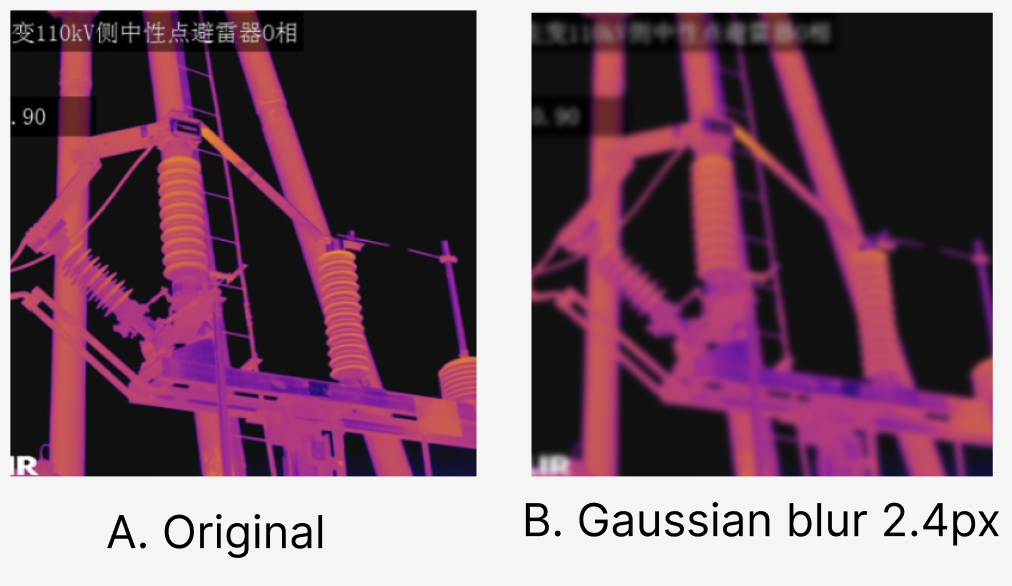
\includegraphics[width=0.6\textwidth]{gambar/bab3/aug-blur.png}
  \caption{\emph{Augmentasi Gaussian Blur} pada dataset dengan \emph{Roboflow}}
  \label{fig:dataset-blur}
\end{figure}

Gambar~\ref{fig:dataset-blur} menunjukkan contoh hasil \emph{augmentasi Gaussian blur} dengan tingkat kekaburan yang bervariasi, mulai dari 0 hingga 2{,}5 piksel. Teknik ini membantu model agar tetap dapat mengenali objek meskipun terdapat gangguan visual minor akibat ketidaksempurnaan sistem pencitraan. Selain itu, diterapkan pula teknik \emph{brightness adjustment} untuk mensimulasikan kondisi pencahayaan yang bervariasi, seperti ketika komponen gardu berada dalam bayangan, terkena cahaya matahari langsung, atau mengalami perubahan intensitas radiasi inframerah karena perubahan suhu lingkungan.

\begin{figure}[H]
  \centering
  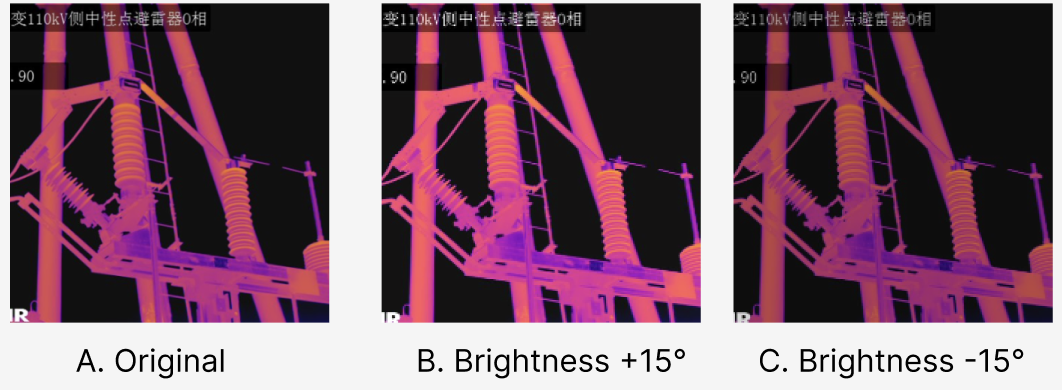
\includegraphics[width=0.85\textwidth]{gambar/bab3/aug-brig.png}
  \caption{\emph{Augmentasi Brightness Adjustment} pada dataset dengan \emph{Roboflow}}
  \label{fig:dataset-brightness}
\end{figure}

Gambar~\ref{fig:dataset-brightness} menunjukkan hasil \emph{brightness adjustment} dengan tingkat kecerahan yang dimodifikasi dari -15\% hingga +15\%. Penyesuaian ini memungkinkan model untuk beradaptasi terhadap dinamika pencahayaan yang umum terjadi di lingkungan luar ruangan, terutama pada pengamatan di area terbuka seperti gardu induk. Teknik selanjutnya adalah \emph{hue adjustment}, yang digunakan untuk menyimulasikan variasi rona warna pada citra termal. Perubahan ini mungkin terjadi akibat pengaruh spektrum inframerah yang berbeda, kalibrasi sensor kamera termal, atau pengaturan palet warna pada perangkat pencitraan.

\begin{figure}[H]
  \centering
  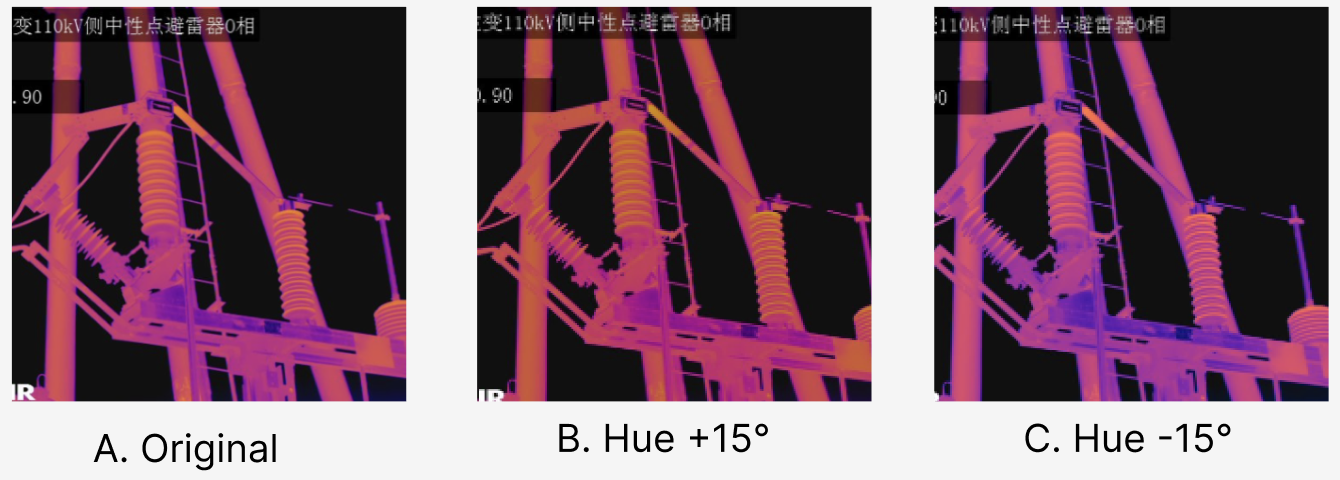
\includegraphics[width=0.85\textwidth]{gambar/bab3/aug-hue.png}
  \caption{\emph{Augmentasi Hue Adjustment} pada dataset dengan \emph{Roboflow}}
  \label{fig:dataset-hue}
\end{figure}

Gambar~\ref{fig:dataset-hue} memperlihatkan hasil \emph{hue adjustment} dengan perubahan rona warna dalam rentang -15\% hingga +15\%. Teknik ini bertujuan agar model tidak terlalu sensitif terhadap perbedaan palet warna termal yang mungkin bervariasi antarsesi akuisisi data atau antarperangkat. Sebagai pelengkap, digunakan juga teknik \emph{horizontal flip} untuk memperkaya perspektif tampilan komponen gardu induk, mengingat orientasi horizontal dapat bervariasi tergantung arah pengambilan citra. Sementara itu, teknik \emph{vertical flip} tidak digunakan karena orientasi vertikal dari komponen-komponen utama seperti transformator, pemutus arus, dan isolator cenderung konstan dan tidak berubah pada kondisi nyata. Dengan menerapkan berbagai teknik \emph{augmentasi} tersebut, model diharapkan dapat mempelajari representasi fitur secara lebih robust dan general, serta mampu melakukan prediksi yang andal meskipun dihadapkan pada kondisi pencitraan yang bervariasi. Pendekatan ini menjadi solusi penting untuk mengatasi keterbatasan jumlah data asli yang dapat dikumpulkan dari lapangan.


\subsubsection{3.3.2.4 Pelatihan Model \emph{YOLOv8}}

Model \emph{YOLOv8} dilatih menggunakan dataset citra termal yang telah melalui proses anotasi, \emph{preprocessing} dan \emph{augmentasi}. Selama proses pelatihan, dilakukan pengaturan terhadap beberapa \emph{hyperparameter} utama, yaitu \emph{batch size}, jumlah \emph{epoch}, dan algoritma \emph{optimizer}, guna memperoleh performa model yang optimal. sedangkan jumlah \emph{epoch} yang diuji bervariasi mulai dari 50, 100, 200, hingga 300. Untuk algoritma optimisasi, dilakukan perbandingan antara \emph{Stochastic Gradient Descent (SGD)} dan \emph{Adam Optimizer} guna melihat pengaruhnya terhadap kecepatan konvergensi dan stabilitas model.  Setelah proses pelatihan selesai, model dievaluasi menggunakan dataset uji yang telah dipisahkan sebelumnya untuk memastikan hasil validasi yang objektif dan menghindari risiko \emph{overfitting}. Evaluasi ini dilakukan dengan mengukur metrik seperti \emph{precision}, \emph{recall}, dan \emph{mAP (mean Average Precision)} guna mengetahui seberapa baik model dapat mendeteksi komponen gardu induk berdasarkan citra termal.


\subsubsection{3.3.2.5 Konversi ke \emph{OpenVINO}}
Setelah model \emph{YOLOv8} dilatih dan tervalidasi, tahap berikutnya adalah melakukan konversi ke format \emph{OpenVINO (Open Visual Inference and Neural Network Optimization)}. Konversi ini bertujuan untuk mengoptimalkan proses inferensi model agar dapat dijalankan secara efisien pada perangkat keras dengan sumber daya terbatas, khususnya yang berbasis CPU.

Dalam penelitian ini, sistem inferensi dirancang untuk dijalankan pada perangkat dengan prosesor Intel, sehingga penggunaan \emph{OpenVINO} menjadi pilihan ideal. \emph{OpenVINO} merupakan toolkit yang dikembangkan oleh Intel untuk mempercepat kinerja model \emph{deep learning} pada arsitektur CPU, GPU, dan VPU Intel. Dengan melakukan konversi model ke format \emph{Intermediate Representation (IR)} yang terdiri dari file \texttt{.xml} dan \texttt{.bin}, model dapat dieksekusi lebih ringan dan cepat, tanpa memerlukan akselerator eksternal seperti GPU.

\subsubsection{3.3.2.6 Inferensi Komponen}

Proses inferensi komponen dilakukan setelah robot tiba pada titik \emph{waypoint} tertentu dan mengambil citra termal menggunakan kamera yang terpasang. Citra tersebut kemudian diproses oleh model deteksi objek \emph{YOLOv8} yang telah dilatih dan dikonversi ke dalam format \emph{OpenVINO} agar dapat berjalan secara efisien di perangkat dengan prosesor Intel. Model ini melakukan deteksi pada citra termal untuk mengidentifikasi dan mengklasifikasikan komponen gardu induk seperti \emph{current transformer}, \emph{circuit breaker}, \emph{bushing}, dan komponen lainnya. Hasil inferensi berupa koordinat \emph{bounding box} dan label kelas dari masing-masing objek yang terdeteksi. Informasi ini digunakan untuk menentukan area citra yang akan dianalisis lebih lanjut, khususnya dalam konteks pemantauan suhu untuk mendeteksi potensi \emph{overheat}. Proses inferensi ini dilakukan secara waktu nyata (\emph{real-time}) dan menjadi dasar bagi tahapan analisis suhu komponen yang lebih spesifik.

\subsubsection{3.3.2.7 Klasifikasi Suhu Komponen}

Setelah komponen berhasil terdeteksi, tahap berikutnya adalah mengklasifikasikan suhu dari masing-masing komponen berdasarkan area \emph{bounding box}. Langkah pertama dalam proses ini adalah mengonversi citra termal ke dalam format \emph{grayscale}, di mana setiap nilai intensitas piksel (0--255) mewakili tingkat suhu relatif. Nilai-nilai ini kemudian dikonversi ke suhu aktual berdasarkan rentang suhu minimum dan maksimum yang dikonfigurasi pada kamera.
Rentang suhu tersebut diperoleh menggunakan protokol ISAPI melalui endpoint \texttt{\emph{GET /ISAPI/Image/channels/<ID>/tempRange}}. Endpoint ini digunakan untuk membaca parameter suhu dari kanal tertentu pada kamera, di mana \texttt{<ID>} mengacu pada nomor kanal kamera termal. Jika permintaan berhasil, kamera akan mengembalikan data dalam format XML yang memuat nilai suhu minimum dan maksimum seperti \ref{lst:xml-example}

\begin{lstlisting}[language=XML, caption={Contoh \emph{XML respone} dari enpoint ISAPI}, label={lst:xml-example}]
  <?xml version="1.0" encoding="utf-8"?>
  <TempRange version="2.0" xmlns="http://www.isapi.org/ver20/XMLSchema">
      <mode>manual</mode>
      <temperatureUpperLimit>100</temperatureUpperLimit>
      <temperatureLowerLimit>20</temperatureLowerLimit>
  </TempRange>
  \end{lstlisting}

Nilai intensitas piksel dalam area \emph{bounding box} kemudian dikonversi ke suhu aktual (\(T\)) menggunakan rumus berikut:

\begin{equation}
T(x, y) = T_{\text{min}} + \left( \frac{I(x, y)}{255} \right) \times (T_{\text{max}} - T_{\text{min}})
\label{eq:suhu-piksel}
\end{equation}


\newpage
dengan keterangan:
\begin{itemize}
  \item \( T(x, y) \): suhu piksel pada posisi \((x, y)\),
  \item \( I(x, y) \): nilai intensitas piksel (0–255),
  \item \( T_{\text{min}} \), \( T_{\text{max}} \): suhu minimum dan maksimum dari kamera.
\end{itemize}

Setelah nilai suhu pada seluruh piksel dalam \emph{bounding box} dihitung, suhu rata-rata komponen ditentukan menggunakan persamaan:

\begin{equation}
T_{\text{avg}} = \frac{1}{N} \sum_{i=1}^{N} T(x_i, y_i)
\label{eq:rata-rata-suhu}
\end{equation}

\noindent
dengan \( N \) adalah jumlah total piksel dalam area komponen. Nilai suhu rata-rata ini kemudian dibandingkan dengan ambang batas tertentu untuk menentukan apakah suatu komponen mengalami suhu berlebih (\emph{overheat}).

\subsection{Implementasi Sistem \emph{Perangkat Lunak Robot}}
Implementasi sistem perangkat lunak robot dilakukan dengan mengembangkan paket-paket ROS yang telah dirancang sebelumnya. Proses ini mencakup pengembangan \emph{IO package}, \emph{mapping package}, \emph{localization package}, \emph{perception package}, dan \emph{autonomy package}. Setiap \emph{package} dikembangkan dengan memperhatikan spesifikasi dan fungsionalitas yang telah ditetapkan pada tahap perancangan.

\subsubsection{3.4.3.1 Implementasi \emph{IO Package}}

\emph{IO package} bertanggung jawab untuk mengelola komunikasi antara robot dan perangkat keras eksternal, dalam hal ini adalah kamera termal. Package ini terdiri dari dua node utama, yaitu \emph{RTSP client} dan \emph{PTZ controller}.  Pada node \emph{RTSP client}, implementasi dilakukan menggunakan pustaka \emph{OpenCV} untuk menangani aliran video dari kamera termal. Node ini terhubung ke kamera melalui protokol \emph{RTSP}, mengambil frame video secara kontinu, dan meneruskannya ke node pada \emph{perception package} untuk proses deteksi objek dan analisis suhu. Selain itu, node ini juga mengelola pengaturan kamera seperti mengubah resolusi menjadi 640$\times$480 piksel, yang merupakan ukuran standar untuk model deteksi objek yang digunakan. Node \emph{PTZ controller} bertugas mengendalikan pergerakan kamera termal, mencakup rotasi (\emph{pan}), kemiringan (\emph{tilt}), dan perbesaran (\emph{zoom}). Node ini menerima perintah dari \emph{Patrol Controller} melalui mekanisme \emph{action}  seperti ditunjukkan pada Gambar~\ref{fig:ptz-control}.

\begin{figure}[H]
  \centering
  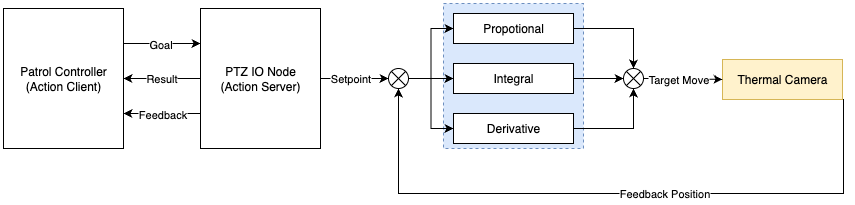
\includegraphics[width=0.8\textwidth]{gambar/bab3/ptz-control.png}
  \caption{Diagram alur kerja \emph{PTZ controller node} dengan kendali \emph{PID}}
  \label{fig:ptz-control}
\end{figure}

Gambar~\ref{fig:ptz-control} menunjukkan alur kerja \emph{PTZ controller node} yang berfungsi untuk menerima perintah dari \emph{Patrol Controller} dalam mengarahkan kamera ke posisi tertentu. Node ini mengimplementasikan kendali umpan balik berbasis \emph{PID controller} guna memastikan pergerakan kamera yang presisi dan stabil. Proses pengendalian ini melibatkan pengukuran posisi aktual kamera, perbandingan terhadap posisi target, serta penyesuaian gerakan berdasarkan selisih (\emph{error}) antara keduanya. Dengan mekanisme tersebut, sistem mampu mengarahkan kamera termal secara otomatis ke komponen gardu induk yang menjadi objek inspeksi. Dalam sistem ini, \emph{Patrol Controller} berperan sebagai \emph{action client}, sedangkan \emph{PTZ IO node} berperan sebagai \emph{action server}. Komunikasi antara keduanya dilakukan melalui mekanisme \emph{action interface} yang mendukung pengiriman \emph{goal}, umpan balik (\emph{feedback}), serta hasil akhir (\emph{result}). Di dalam \emph{PTZ IO node}, diterapkan kendali umpan balik menggunakan algoritma \emph{PID} untuk mengatur pergerakan kamera menuju posisi target secara akurat dan responsif.

Selisih antara posisi target (\emph{setpoint}) dan posisi aktual digunakan sebagai \emph{error}, yang kemudian diproses oleh tiga komponen utama dalam kendali \emph{PID}, yaitu: komponen \emph{proportional} yang memberikan respon proporsional terhadap \emph{error} saat ini; komponen \emph{integral} yang mengakumulasi \emph{error} dari waktu ke waktu untuk mengoreksi kesalahan jangka panjang; serta komponen \emph{derivative} yang berfungsi sebagai peredam terhadap perubahan \emph{error} yang tiba-tiba. Untuk meningkatkan stabilitas dan respons sistem, algoritma \emph{PID} yang diterapkan menggunakan pendekatan \emph{region-based gain tuning}, yaitu pembagian ruang \emph{error} menjadi beberapa wilayah atau \emph{region}, masing-masing dengan nilai parameter $K_p$, $K_i$, dan $K_d$ yang berbeda. Misalnya, ketika nilai \emph{error} cukup besar (melebihi ambang batas tertentu), digunakan parameter penguatan yang lebih agresif untuk mempercepat konvergensi; sebaliknya, saat \emph{error} kecil, digunakan parameter yang lebih konservatif untuk menghindari osilasi dan menjaga kestabilan.Selain itu, sistem juga mempertimbangkan nilai keluaran minimum dan maksimum dari kontrol untuk menjaga agar perintah gerakan tidak melebihi batas fisik aktuator kamera. Mekanisme ini membantu sistem beradaptasi terhadap dinamika yang berbeda dalam proses penyesuaian posisi kamera.

\vspace{1ex}
\begin{algorithm}[H]
\caption{Region-Based PID Controller with Membership Levels}
\label{alg:region-pid}
\KwIn{\emph{setpoint}, \emph{actual\_position}, \emph{prev\_error}, \emph{accum\_error}}
\KwData{PID arrays: $K_P[i], K_I[i], K_D[i]$; bounds: $output\_bound$, $accum\_bound$; $membership\_amount$}
\KwOut{\emph{control\_output}}

$error \gets setpoint - actual\_position$\;

$step \gets \dfrac{output\_bound}{membership\_amount}$\;
$idx \gets \min(membership\_amount - 1,\ \left\lfloor \dfrac{|error|}{step} \right\rfloor)$\;

$K_p \gets K_P[idx]$\;
$K_i \gets K_I[idx]$\;
$K_d \gets K_D[idx]$\;

$accum\_error \gets \texttt{clamp}(accum\_error + error,\ -accum\_bound,\ accum\_bound)$\;
$derivative \gets error - prev\_error$\;

$output \gets K_p \cdot error + K_i \cdot accum\_error + K_d \cdot derivative$\;
$output \gets \texttt{clamp}(output,\ -output\_bound,\ output\_bound)$\;

$prev\_error \gets error$\;
\Return $output$\;
\end{algorithm}



Logika pengendalian tersebut dirangkum secara rinci dalam Algoritma~\ref{alg:region-pid}, yang menggambarkan proses komputasi sinyal kendali berdasarkan \emph{error} saat ini, serta pemilihan parameter kendali yang disesuaikan dengan besar kecilnya \emph{error} melalui pendekatan \emph{region-based gain tuning}.



\subsubsection{3.2.3.2 Implementasi Sistem \emph{Localization and Mapping Package}}

Implementasi sistem \emph{Localization and Mapping Package} dalam penelitian ini dirancang untuk mendukung fleksibilitas terhadap berbagai kondisi operasional di lapangan. Sistem dibangun secara modular dengan integrasi empat metode utama yang dapat diaktifkan melalui konfigurasi parameter pada berkas \texttt{launch} di ROS. Keempat metode tersebut terbagi ke dalam dua kelompok, yaitu metode berbasis \emph{odometry-only} dan metode berbasis \emph{SLAM}. Pada kelompok pertama, metode \emph{FastLIO2} dan \emph{DLIO} digunakan untuk melakukan estimasi posisi robot secara langsung tanpa membentuk peta lingkungan. Masing-masing metode dijalankan sebagai \emph{node} ROS terpisah, yang menerima masukan berupa data \emph{point cloud} dari empat sensor \emph{LiDAR Livox Mid-360} serta data orientasi dan akselerasi dari sensor \emph{Yesense-IMU}. Hasil estimasi posisi dipublikasikan dalam sistem transformasi ROS melalui \emph{tf broadcaster} dan dapat digunakan oleh subsistem lain seperti navigasi dan kontrol. Namun, pada saat implementasi, metode \emph{DLIO} tidak dapat dijalankan secara fungsional pada platform robot yang digunakan. Hal ini disebabkan oleh ketidaksesuaian \emph{timestamp} antara data \emph{LiDAR} dan \emph{IMU}, sedangkan \emph{DLIO} mensyaratkan sinkronisasi waktu yang presisi untuk melakukan \emph{sensor fusion}. Ketidaksesuaian tersebut mengakibatkan kegagalan pemrosesan internal pada \emph{node} \emph{DLIO}, sebagaimana ditunjukkan pada Gambar~\ref{fig:dlio-error}.

\begin{figure}[H]
  \centering
  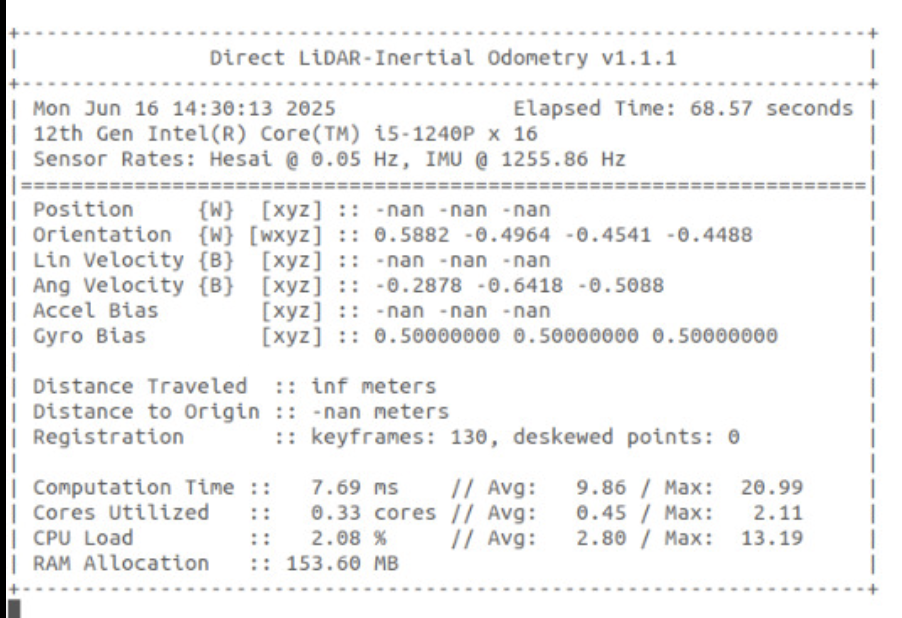
\includegraphics[width=0.6\textwidth]{gambar/bab3/dlio-error-negate.png}
  \caption{Kegagalan inisialisasi \emph{DLIO} akibat ketidaksesuaian \emph{timestamp}} 
  \label{fig:dlio-error}
\end{figure}

Gambar~\ref{fig:dlio-error} menunjukkan pesan kesalahan yang muncul saat mencoba menjalankan \emph{node} \emph{DLIO} dimana \emph{position} menjadi \emph{nan}. Pesan ini mengindikasikan bahwa data dari sensor \emph{LiDAR} dan \emph{IMU} tidak dapat disinkronkan dengan benar, sehingga proses estimasi posisi tidak dapat dilanjutkan. Akibatnya, implementasi metode \emph{DLIO} tidak dapat digunakan dalam sistem robot ini. Metode \emph{FastLIO2} diimplementasikan dengan memanfaatkan pustaka ROS yang telah tersedia dan diintegrasikan dengan sensor \emph{LiDAR} dan \emph{IMU} pada robot. Metode ini telah dioptimalkan untuk berjalan pada platform dengan sumber daya terbatas, seperti yang digunakan dalam penelitian ini. \emph{FastLIO2} berhasil diimplementasikan dan mampu beroperasi secara \emph{real-time} untuk mengestimasi posisi berdasarkan data \emph{point cloud} dari sensor \emph{LiDAR}. Estimasi posisi dihitung menggunakan algoritma \emph{LiDAR-Inertial Odometry}, dengan dukungan data dari \emph{IMU} untuk meningkatkan akurasi. Pada kelompok metode kedua yang berbasis \emph{SLAM}, implementasi dilakukan dengan pendekatan \emph{frontend-backend}. Pada metode ketiga, proses pemetaan dilakukan terlebih dahulu menggunakan \emph{FastLIO2} untuk membentuk peta dua dimensi dalam format \emph{grid map}. Peta ini kemudian dimuat oleh \emph{node} \emph{HDL Localization}, yang melakukan pelokalan secara \emph{real-time} dengan mencocokkan data \emph{point cloud} terhadap peta. Estimasi posisi robot dipublikasikan dalam bentuk transformasi dari kerangka \texttt{map} ke \texttt{base\_link} melalui sistem \emph{tf} ROS.

Metode keempat, yaitu \emph{Fast-LIO-SAM}, menggabungkan estimasi \emph{LiDAR-Inertial Odometry} pada bagian \emph{frontend} dengan proses optimisasi graf berbasis \emph{Smoothing and Mapping (SAM)} pada bagian \emph{backend}. Selama proses pemetaan, data dari sensor direkam dalam format file \texttt{.bag} dan digunakan secara \emph{offline} oleh \emph{node} \emph{Fast-LIO Localization QN} untuk melakukan estimasi posisi. Node ini mencocokkan data \emph{point cloud} terbaru dengan peta yang telah terbentuk untuk memperkirakan posisi robot, kemudian menerbitkannya melalui \emph{tf broadcaster}. 


\subsubsection{3.4.3.3 Implementasi Sistem \emph{Perception Package}}

\emph{Perception package} bertanggung jawab untuk mendeteksi dan menganalisis komponen gardu induk berdasarkan citra termal dari kamera, serta mendeteksi rintangan di sekitar robot. Package ini terdiri dari dua node utama, yaitu \emph{Object Detection} dan \emph{Obstacle Detector}. Node \emph{Object Detection} mengimplementasikan model deteksi objek \emph{YOLOv8} yang telah dijelaskan pada bagian sebelumnya. Sementara itu, node \emph{Obstacle Detector} menggunakan algoritma \emph{Braitenberg Vehicle} untuk mendeteksi rintangan berdasarkan data dari sensor \emph{LiDAR}. Algoritma ini membagi area di depan robot menjadi 32 \emph{segment}. Setiap \emph{segment} dianalisis berdasarkan jarak terdekat yang terdeteksi oleh sensor \emph{LiDAR}. Jika jarak pada suatu \emph{segment} lebih kecil dari ambang batas tertentu, maka \emph{segment} tersebut dianggap sebagai rintangan. Informasi ini kemudian dikirimkan ke node \emph{Patrol Controller} untuk pengambilan keputusan pergerakan secara dinamis.

\begin{figure}[H]
  \centering
  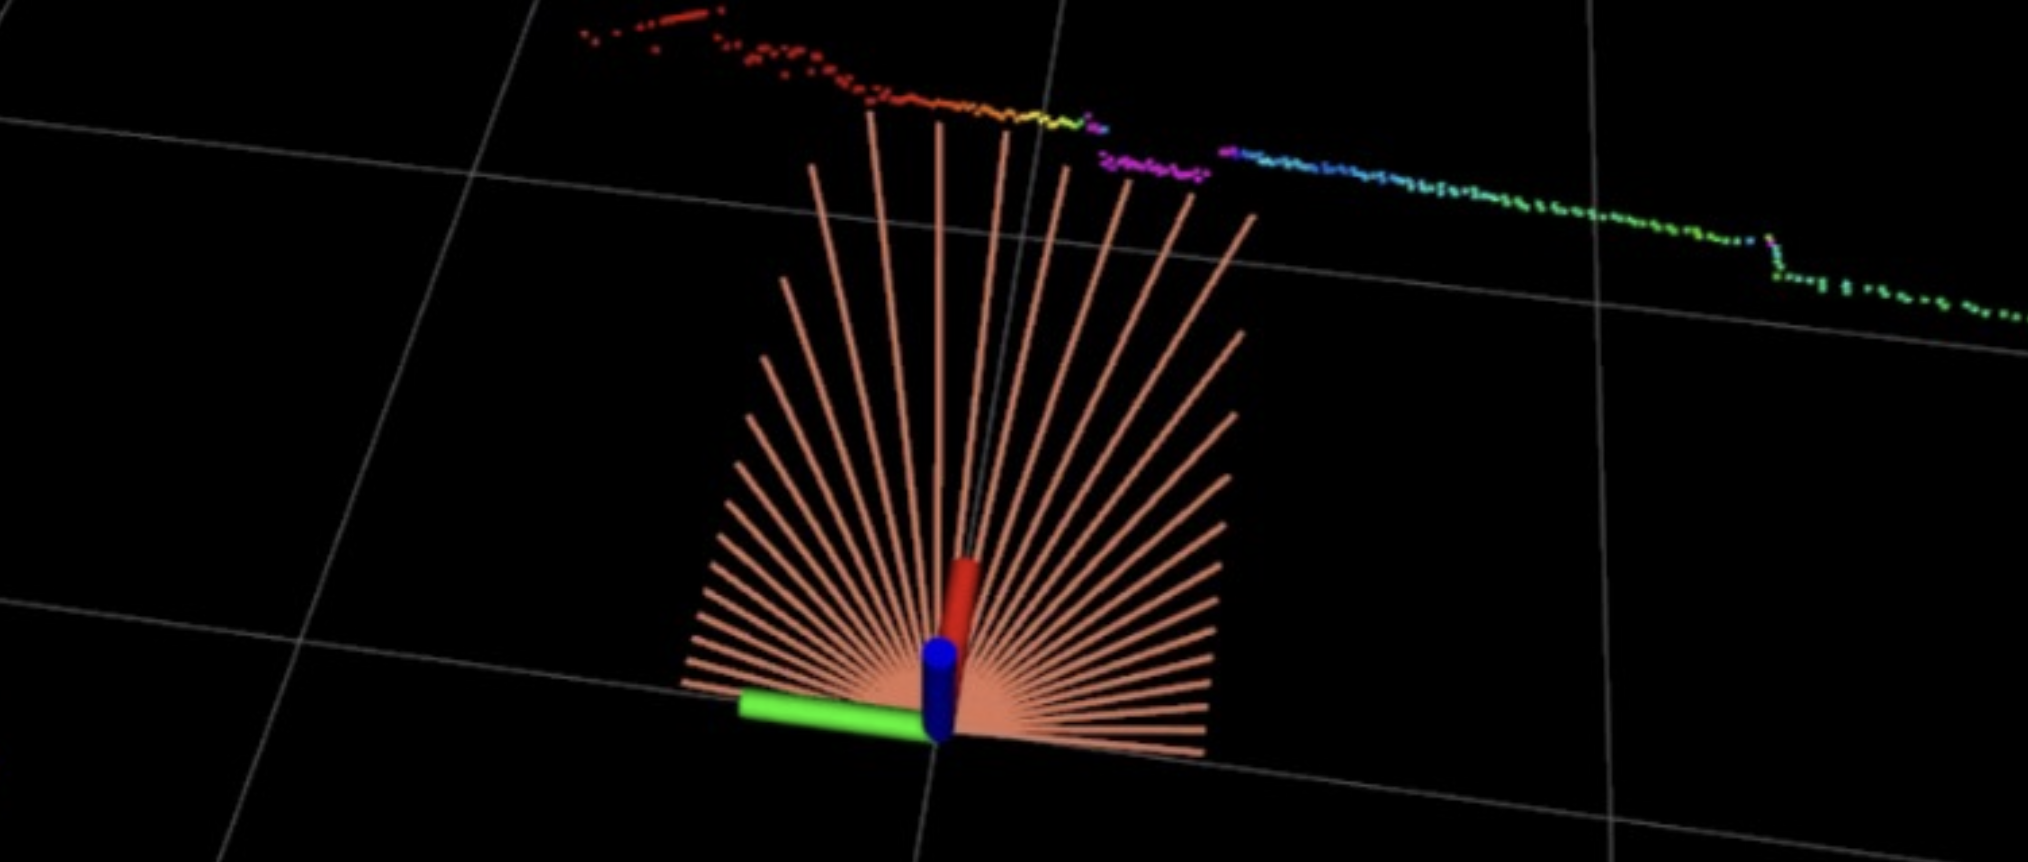
\includegraphics[width=0.6\textwidth]{gambar/bab3/obstacle_avoidance.png}
  \caption{Implementasi \emph{Obstacle Detector} dengan LiDAR}
  \label{fig:obstacle-detector}
\end{figure}

Gambar~\ref{fig:obstacle-detector} memperlihatkan visualisasi hasil pembacaan LiDAR yang dibagi ke dalam 32 arah atau segmen (garis merah) di depan robot. Setiap garis mewakili arah pemindaian, sedangkan titik-titik warna di kejauhan merupakan objek yang terdeteksi. Data ini digunakan untuk menentukan apakah ada rintangan yang perlu dihindari berdasarkan jaraknya terhadap robot. Data dari \emph{node} ini kemudian digabungkan dalam \emph{Patrol Controller} untuk menentukan tindakan yang harus diambil, baik itu melanjutkan pergerakan, menghindari rintangan, atau melakukan inspeksi komponen gardu induk. 


\subsubsection{3.4.3.4 Implementasi Sistem \emph{Autonomy Package}}

Proses navigasi robot dilakukan dengan mengikuti jalur waypoint menggunakan algoritma \emph{Pure Pursuit} dan kontrol kecepatan berbasis \emph{PID controller}. Sistem ini juga memiliki kemampuan untuk melakukan inspeksi komponen secara otomatis ketika mencapai waypoint bertipe inspeksi, serta menghindari rintangan secara dinamis berdasarkan arsitektur perilaku (\emph{behavior-based arbitration}).

\begin{algorithm}[H]
  \caption{Navigasi Waypoint dengan Pure Pursuit dan Subsumption Architecture}
  \label{alg:patrol-controller}
  \KwIn{Daftar \texttt{waypoints[]} dengan atribut \texttt{position, type}}
  \KwOut{Navigasi dan inspeksi otomatis oleh robot}
  $i \gets 0$\;
  \While{$i < \texttt{waypoints.length}$}{
      $\mathbf{w}_i \gets \texttt{waypoints}[i]$\;
      
      \While{\textbf{not} \texttt{isAtWaypoint}($\mathbf{w}_i$)}{
          \uIf{\texttt{detectObstacle()}}{
              \texttt{avoidObstacleBehavior()}\;
          }
          \Else{
              Hitung sudut arah relatif:\;
              
              $\alpha \gets \arctan2(y_{\text{target}} - y, x_{\text{target}} - x) - \theta$\;
  
              Hitung sudut kemudi:\;
              
              $\delta \gets \arctan\left(\frac{2L \sin \alpha}{L_d}\right)$\;
  
              Hitung error kecepatan:\;
  
              $e_v(t) \gets v_{\text{target}} - v(t)$\;
  
              $v_{\text{cmd}} \gets K_p^v e_v(t) + K_i^v \int_0^t e_v(\tau)\, d\tau + K_d^v \frac{de_v(t)}{dt}$\;
  
              Hitung error arah:
  
              $e_\delta(t) \gets \delta - \delta(t)$\;
  
              $\omega_{\text{cmd}} \gets K_p^\delta e_\delta(t) + K_i^\delta \int_0^t e_\delta(\tau)\, d\tau + K_d^\delta \frac{de_\delta(t)}{dt}$\;
  
              \texttt{publish}($v_{\text{cmd}}, \omega_{\text{cmd}}$)\;
          }
      }
  
      \If{$\mathbf{w}_i.\text{\texttt{type}} == \texttt{"inspection"}$}{
          $\texttt{ptz\_pose} \gets \texttt{getPTZPose}(\mathbf{w}_i)$\;
          
          \texttt{sendToPTZNode(ptz\_pose)}\;
          
          \texttt{sendCommandToCV("capture")}\;
  
          \uIf{\texttt{waitForCVResponse()} == \texttt{"success"}}{
              Lanjut ke waypoint berikutnya\;
          }
      }
      $i \gets i + 1$\;
  }
  \textbf{Navigasi selesai}\;
  \end{algorithm}
  

Algoritma~\ref{alg:patrol-controller} menggambarkan alur navigasi robot dalam mengikuti daftar waypoint yang diberikan. Proses ini dilakukan dengan dua komponen utama: pergerakan menuju waypoint menggunakan algoritma \emph{Pure Pursuit}, serta penghindaran rintangan berdasarkan arsitektur perilaku \emph{subsumption}.  Pada setiap iterasi, robot memeriksa apakah terdapat rintangan di jalurnya. Jika terdeteksi, sistem segera mengaktifkan perilaku penghindaran rintangan secara prioritas. Jika tidak, robot menghitung sudut arah relatif terhadap target (\(\alpha\)), sudut kemudi (\(\delta\)), serta menghasilkan perintah kecepatan linier dan sudut (\(v_{\text{cmd}}\) dan \(\omega_{\text{cmd}}\)) melalui kendali \emph{PID} untuk menjaga kestabilan gerak dan presisi arah. Ketika mencapai waypoint bertipe \texttt{inspection}, sistem akan mengarahkan kamera PTZ dan menjalankan proses pengambilan gambar menggunakan \emph{Computer Vision}. Dengan struktur algoritma ini, sistem navigasi mampu melakukan perpindahan antar waypoint secara otonom sekaligus menjalankan inspeksi otomatis dan penghindaran rintangan secara reaktif.


\subsection{Implementasi Sistem \emph{Control Station}}
Sistem \emph{Control Station} diimplementasikan sebagai antarmuka pengguna berbasis web yang memungkinkan operator untuk mengendalikan robot, memantau statusnya, dan mengakses data yang dikumpulkan selama operasi. Implementasi sistem ini dapat dibagi menjadi dua komponen utama yaitu\emph{front-end} dan \emph{back-end}.

\subsubsection{3.4.4.1 Implementasi \emph{Frontend}}
\emph{Frontend} dari sistem ini dibuat menggunakan \emph{library} \emph{React} dan \emph{framework} \emph{Next.js} untuk memberikan pengalaman pengguna yang cepat dan dinamis. Pemilihan \emph{React} didasarkan pada prinsip \emph{component-based architecture} yang memungkinkan pembuatan antarmuka pengguna dengan komponen-komponen modular yang dapat digunakan kembali. Hal ini mempercepat proses pengembangan dan mengurangi redundansi kode, karena pengembang dapat memanfaatkan kembali komponen yang sudah ada di berbagai bagian aplikasi. Sementara itu, \emph{Next.js} memperluas kemampuan \emph{React} dengan menambahkan fitur seperti \emph{server-side rendering} (SSR), \emph{static site generation}, dan \emph{routing} berbasis berkas. Dengan menggunakan \emph{Next.js}, sistem ini dapat menghasilkan halaman yang lebih cepat dengan waktu pemuatan yang lebih singkat karena SSR memungkinkan konten halaman di-\emph{render} di sisi \emph{server} sebelum dikirimkan ke \emph{klien}.

Untuk pengelolaan \emph{state}, sistem ini menggunakan \emph{state management} dengan \emph{Zustand}, sebuah \emph{library} ringan dan efisien yang memungkinkan pengelolaan \emph{state} secara sederhana dan terpusat tanpa memerlukan \emph{boilerplate code} seperti yang banyak muncul pada penggunaan \emph{reducer}. Untuk pengambilan data dari \emph{server}, aplikasi ini menggunakan \emph{Tanstack Query}, yang mempermudah pengelolaan data, mendukung \emph{caching}, dan menyediakan pembaruan data secara otomatis ketika ada perubahan. Sistem ini juga mengimplementasikan \emph{client-side filtering} dan \emph{server-side pagination}. \emph{Client-side filtering} memungkinkan data yang ditampilkan untuk difilter langsung di sisi \emph{klien}, mempercepat proses pencarian, sementara \emph{server-side pagination} membagi data menjadi beberapa halaman, sehingga hanya sebagian data yang dimuat pada satu waktu, mengurangi beban pada \emph{server} dan meningkatkan kinerja aplikasi. \emph{Server-side rendering} (SSR) yang didukung oleh \emph{Next.js} memungkinkan aplikasi untuk me-\emph{render} halaman di sisi \emph{server} sebelum mengirimkannya ke \emph{klien}, sehingga mempercepat waktu pemuatan halaman dan meningkatkan kemampuan mesin pencari untuk mengindeks halaman dengan lebih baik.

Untuk tampilan antarmuka pengguna (UI), aplikasi ini menggunakan \emph{Shadcn UI} dan \emph{Tailwind CSS}. \emph{Shadcn UI} adalah pustaka komponen UI yang menyediakan elemen-elemen desain minimalis dan responsif, sementara \emph{Tailwind CSS} memungkinkan pengembang untuk mendesain elemen-elemen UI dengan cepat menggunakan \emph{utility-first CSS}, sehingga memudahkan pembuatan tampilan yang responsif dan dinamis. Untuk manajemen autentikasi, aplikasi ini menggunakan \emph{cookies} untuk menyimpan \emph{token} autentikasi pengguna. Dengan menggunakan \emph{cookies}, sesi pengguna dapat dipertahankan meskipun terjadi \emph{refresh} halaman. \emph{Cookies} ini bekerja dengan \emph{token JWT} untuk memverifikasi identitas pengguna dalam setiap permintaan ke \emph{server}. Berikut merupakan implementasi tampilan antarmuka pengguna pada \emph{control station} yang telah dirancang sebelumnya.

\subsubsection{3.4.4.2 Implementasi Sistem \emph{Backend}}

Sistem \emph{backend} dari aplikasi ini dibuat menggunakan bahasa pemrograman \emph{TypeScript} dengan \emph{framework} \emph{Express.js} untuk membangun \emph{RESTful API} yang efisien dan mudah diakses. \emph{TypeScript} dipilih karena memberikan keunggulan dalam hal tipe data, yang memungkinkan pengembang untuk menulis kode yang lebih aman dan mudah dipelihara. Dengan menggunakan \emph{Express.js}, pengembangan \emph{API} menjadi lebih cepat dan mudah, karena \emph{framework} ini menyediakan berbagai fitur yang dibutuhkan untuk membangun aplikasi web dan \emph{API} secara efisien. Untuk pengelolaan basis data, sistem ini menggunakan pustaka \emph{Sequelize} sebagai \emph{Object-Relational Mapping} (ORM). \emph{Sequelize} memungkinkan interaksi dengan basis data menggunakan model \emph{JavaScript} yang lebih mudah dipahami dan dikelola, tanpa perlu menulis kueri \emph{SQL} secara langsung. ORM ini menyediakan berbagai fitur seperti validasi data, relasi antar tabel, serta sistem migrasi untuk mempermudah pengelolaan skema dan konsistensi data aplikasi.

Dalam hal autentikasi, sistem menerapkan pendekatan berbasis \emph{JWT} (\emph{JSON Web Tokens}) untuk \emph{login} dan pengelolaan sesi. Pengguna yang berhasil melakukan autentikasi akan menerima \emph{access token} dan \emph{refresh token}. \emph{Access token} digunakan untuk mengakses \emph{endpoint API} yang bersifat privat, sedangkan \emph{refresh token} memungkinkan pembaruan \emph{access token} yang telah kedaluwarsa tanpa perlu \emph{login} ulang. \emph{Middleware} \emph{auth} digunakan untuk memverifikasi setiap token yang masuk dalam permintaan \emph{API}, sehingga hanya pengguna yang telah terautentikasi yang dapat mengakses sumber daya tertentu. Sistem ini juga menerapkan \emph{Role-Based Access Control} (RBAC) untuk membatasi hak akses berdasarkan peran pengguna, seperti \emph{superadmin}, \emph{admin}, atau \emph{user}. Selain itu, fitur keamanan lintas domain dikendalikan melalui penerapan mekanisme \emph{CORS} (\emph{Cross-Origin Resource Sharing}), yang memastikan bahwa hanya domain yang sah dan terverifikasi yang dapat berinteraksi dengan sistem \emph{API backend}.

Untuk mendukung pengolahan data secara waktu nyata (\emph{real-time}), sistem ini menggunakan protokol \emph{WebSocket}. Dengan \emph{WebSocket}, koneksi dua arah (\emph{full-duplex}) antara \emph{klien} dan \emph{server} dapat terjaga secara terus-menerus, memungkinkan pengiriman data seperti posisi robot, status sensor, dan notifikasi sistem secara langsung tanpa perlu melakukan permintaan berulang (\emph{polling}). Pendekatan ini sangat penting untuk sistem pemantauan dan kontrol yang memerlukan latensi rendah dan pembaruan data secara instan. Sementara itu, untuk mendukung transmisi video langsung dari kamera robot ke antarmuka pengguna, sistem menggunakan protokol \emph{WebRTC} (\emph{Web Real-Time Communication}). \emph{WebRTC} memungkinkan komunikasi audio dan video secara \emph{peer-to-peer} antara \emph{klien} dan \emph{server}, tanpa perlu \emph{plugin} tambahan, serta mendukung kompresi dan pengiriman media dengan efisiensi tinggi. Penggunaan \emph{WebRTC} memastikan bahwa tayangan video dari kamera robot dapat diakses secara langsung (\emph{live streaming}) dengan latensi rendah dan kualitas yang dapat disesuaikan secara adaptif sesuai kondisi jaringan.

\section{Integrasi Sistem}
Integrasi sistem dilakukan dengan menggabungkan seluruh komponen perangkat keras dan perangkat lunak yang telah dirancang untuk menciptakan sistem yang berjalan secara efisien dan terkoordinasi. Tahap pertama adalah integrasi komponen elektrikal, yang melibatkan pemasangan perangkat tambahan seperti kamera termal, router nirkabel, dan perangkat \emph{switch} jaringan pada robot. Komponen-komponen ini dihubungkan dengan catu daya 24 VDC dari port daya \emph{navigation host} robot, memastikan semua perangkat dapat beroperasi tanpa memerlukan sumber daya eksternal tambahan. Selanjutnya, perangkat-perangkat ini dikonfigurasi dalam jaringan lokal dengan alamat IP statis, memungkinkan komunikasi antar perangkat di dalam robot untuk mendukung fungsionalitas sistem. Untuk komunikasi antara \emph{control station} dan robot, digunakan skema komunikasi nirkabel \emph{Point-to-Point} (PTP). Pada \emph{control station}, router berfungsi sebagai \emph{access point} (AP) yang terhubung ke jaringan lokal robot. Sementara itu, pada robot, perangkat \emph{router} berfungsi sebagai \emph{station}, yang terhubung langsung dengan \emph{access point} yang ada di \emph{control station}. Konfigurasi ini memungkinkan pertukaran data dua arah berkecepatan tinggi antara robot dan \emph{control station}, dengan latensi rendah yang sangat krusial untuk mendukung transmisi data secara \emph{real-time}.

Setelah integrasi perangkat keras, sistem \emph{ROS} (Robot Operating System) diimplementasikan pada robot untuk mengelola komunikasi antar \textit{package} dan menjalankan berbagai fungsionalitas robot. ROS mengatur deteksi objek menggunakan model \emph{YOLO}, navigasi otonom, serta pemantauan suhu untuk mendeteksi potensi \emph{overheat}. Sistem ini memungkinkan integrasi komponen perangkat keras dan perangkat lunak dalam robot, dengan \emph{package}-package yang saling terhubung dan berkomunikasi untuk mencapai tujuan operasi otonom yang efisien.

Setelah robot terintegrasi dengan sistem ROS, \emph{control station} yang berbasis web diimplementasikan pada PC operator. \emph{Control station} memungkinkan operator untuk memantau dan mengendalikan robot secara \emph{real-time}, dengan antarmuka pengguna yang menyediakan akses mudah untuk memantau posisi robot, status sensor, dan hasil deteksi suhu berlebih pada komponen gardu induk. Di dalam \emph{control station}, operator dapat memasukkan data komponen gardu induk, termasuk jenis, lokasi, dan ambang batas suhu abnormal, yang kemudian terintegrasi dengan sistem. Dengan demikian, robot dan seluruh komponen gardu dapat terdaftar dan dipantau secara terpusat dalam satu sistem, yang memudahkan pengawasan dan pengendalian operasi robot di lapangan.

\section{Alur Kerja Sistem}

Alur kerja sistem dalam penelitian ini mencakup integrasi data komponen gardu induk, pembuatan rute, penentuan waypoint pada robot, serta pengaturan jadwal patroli yang terhubung dengan sistem \emph{control station}. Selain itu, terdapat pula mekanisme koreksi navigasi robot menggunakan metode \emph{Fast-LIO2} dan penghindaran rintangan untuk memastikan robot tetap pada jalur yang telah ditentukan. Proses ini dimulai dengan pengaturan data komponen hingga pengoperasian robot untuk patroli dan deteksi suhu berlebih pada komponen gardu induk. Berikut adalah penjelasan alur kerja secara rinci:

\subsection{Integrasi Data Komponen Gardu Induk}
Pada tahap awal, \emph{control station} menerima data komponen gardu induk yang mencakup informasi tentang nama kelas komponen, ambang batas suhu, serta posisi komponen yang terpasang di gardu induk. Data ini digunakan sebagai dasar bagi robot untuk mendeteksi suhu berlebih pada komponen gardu induk selama proses patroli. 

\subsection{Pembuatan Rute dan Waypoint di \emph{Control Station}}
Setelah data komponen terintegrasi, operator dapat membuat rute patroli di \emph{control station}. Rute ini terdiri dari serangkaian waypoint yang masing-masing berisi informasi tentang lokasi (X, Y), orientasi (Z), serta jenis waypoint (seperti \emph{start}, \emph{scan area}, atau \emph{dock charge}). Data waypoint ini kemudian dikirimkan ke robot dan digunakan untuk navigasi. Pada setiap waypoint, terdapat parameter tambahan yang digunakan untuk mengontrol pergerakan robot dan pengaturan kamera, seperti kecepatan (\emph{speed}), tipe gait (\emph{gaitType}), serta kontrol kamera seperti pan, tilt, dan zoom. Parameter ini memungkinkan robot untuk bergerak sesuai dengan yang diinginkan serta melakukan pemindaian atau deteksi suhu pada komponen gardu induk. Berikut adalah contoh format salah satu array waypoint yang digunakan dalam sistem:

\begin{lstlisting}[language=XML, caption={Sample Waypoint JSON Data}, label={lst:waypoint-example}]
  {
    "id": 6,
    "sequenceOrder": 0,
    "locationX": 10.5,
    "locationY": 20.3,
    "orientationZ": 45,
    "waypointType": "start",
    "gaitType": "walk",
    "speed": 0.5,
    "bodyHeight": 1.2,
    "cameraPan": 90,
    "cameraTilt": -10,
    "rgbCameraZoom": 1.5,
    "thermalCameraZoom": 2,
    "direction": "forward",
    "useObstacleAvoidance": true,
    "map": "route_1"
  }
  \end{lstlisting}

\subsection{Navigasi Robot}
Setelah waypoint dan rute ditentukan, robot dapat dijadwalkan untuk patroli pada waktu tertentu. Robot yang selalu terhubung dalam kondisi docking station akan melanjutkan patroli ke rute yang telah ditentukan pada waktu yang telah dijadwalkan. Selama patroli, robot bergerak menuju setiap waypoint secara berurutan, dengan mempertimbangkan kecepatan dan metode pergerakan yang telah diatur. Jika robot mendeteksi suhu berlebih pada komponen gardu induk, sistem akan melaporkan kondisi tersebut ke \emph{control station}.

\subsection{Deteksi Overheat dan Visualisasi pada \emph{Control Station}}
Robot dilengkapi dengan sistem deteksi suhu menggunakan kamera termal untuk memantau suhu komponen gardu induk. Jika robot mendeteksi adanya komponen yang mengalami suhu berlebih, kondisi tersebut akan dikirimkan ke \emph{control station}. Di \emph{control station}, informasi suhu berlebih akan divisualisasikan, dengan memperhitungkan posisi robot dan kelas komponen yang terdeteksi. Visualisasi ini memungkinkan operator untuk mengambil langkah segera jika terjadi overheat.

\subsection{Koreksi Posisi dengan \emph{Fast-LIO2}}
Selama patroli, robot dapat mengalami penyimpangan posisi atau kesalahan dalam estimasi lokasi akibat faktor lingkungan, misalnya perubahan medan atau ketidakakuratan sensor. Oleh karena itu, robot dilengkapi dengan \emph{Fast-LIO2} yang digunakan untuk memperbaiki posisi robot. Sistem ini mengintegrasikan data dari sensor LiDAR dan IMU untuk memperkirakan posisi robot secara akurat. Prediksi posisi robot pada waktu \( t \) dihitung menggunakan data IMU, sedangkan pencocokan data LiDAR dengan peta digunakan untuk memperbaiki estimasi posisi tersebut. Proses koreksi posisi ini dapat dijelaskan dengan persamaan berikut:

\begin{equation}
\mathbf{x}_t^{\text{updated}} = \mathbf{x}_t^{\text{pred}} + \mathbf{K} \cdot (\mathbf{z}_t - h(\mathbf{x}_t^{\text{pred}}))
\end{equation}

Di sini, \( \mathbf{x}_t^{\text{pred}} \) adalah posisi robot yang diprediksi berdasarkan data IMU, \( \mathbf{z}_t \) adalah data pengukuran LiDAR, dan \( \mathbf{K} \) adalah matriks gain dari pembaruan Kalman. Fungsi \( h(\mathbf{x}_t^{\text{pred}}) \) adalah model yang menghubungkan prediksi posisi robot dengan data pengukuran LiDAR. Proses koreksi posisi ini memungkinkan robot untuk memperbaiki estimasi posisi secara real-time dan menjaga akurasi navigasi.

\subsection{Penghindaran Rintangan dan Kembali ke Jalur}
Jika robot mendeteksi adanya rintangan selama patroli, sistem \emph{obstacle avoidance} akan mengaktifkan algoritma penghindaran untuk menghindari hambatan tersebut. Setelah rintangan terhindar, robot akan melanjutkan perjalanannya dan kembali ke jalur semula menggunakan \emph{Fast-LIO2} untuk memastikan robot tetap pada jalur yang telah ditentukan. Jika robot masih menyimpang setelah menghindari rintangan, sistem akan mengoreksi posisi dan arah robot untuk memastikan kembali ke jalur yang benar. Penghindaran rintangan diaktifkan secara otomatis melalui deteksi objek yang ada di sekitar robot. Data dari sensor LiDAR yang dipasang pada robot digunakan untuk mendeteksi objek di sekitarnya, dan algoritma \emph{Braitenberg} digunakan untuk menilai seberapa dekat objek dengan robot. Jika jarak objek terdeteksi lebih kecil dari ambang batas yang telah ditentukan, robot akan menyesuaikan jalurnya dan menghindari rintangan.

\subsection{Pengecekan Konfigurasi dan Kembali ke Posisi Awal}
Pada saat robot melakukan docking untuk pengisian daya, sistem akan memeriksa dan memperbarui konfigurasi yang diterima dari \emph{control station}. Perubahan konfigurasi, baik itu rute atau jadwal patroli, hanya dapat dilakukan ketika robot berada dalam kondisi \emph{idle} atau saat berada di \emph{dock station}. Hal ini memastikan bahwa perubahan tidak mengganggu patroli yang sedang berjalan. Setelah menyelesaikan patroli, robot akan kembali ke posisi awalnya. Rute yang telah dibuat harus mencakup titik awal dan titik akhir yang sama, sehingga robot dapat kembali ke tempat yang sama setelah menyelesaikan patroli. Dalam hal ini, sistem memastikan bahwa robot mengikuti jalur yang benar, melakukan koreksi posisi jika diperlukan, dan kembali ke titik awal setelah menyelesaikan tugasnya. Dengan alur kerja yang terstruktur ini, robot dapat melakukan patroli secara otomatis, memantau kondisi komponen gardu induk, dan mengatasi potensi overheat yang terjadi.
